\chapter{Optics}


\section{Reflection and Mirrors}

\textbf{Worked example: a mirror image.} A concave mirror has focal length $f = 10$ cm. An object is $30$ cm away. The mirror equation $\frac{1}{f} = \frac{1}{d_o} + \frac{1}{d_i}$ gives $\frac{1}{d_i} = \frac{1}{10} - \frac{1}{30} = \frac{2}{30}$, so $d_i = 15$ cm.

No object reflects every photon, but a mirror is pretty close. Let us
talk about reflections in a mirror.\index{mirror}

\section{Reflection}
A mirror is a sheet of glass with a thin layer of metal, usually silver or
aluminum, on its back. Metals contain many electrons that are free to move.
When light reaches the metal, these electrons vibrate and send nearly all of
the light back out.

The smoothness of the surface decides what you see. On a mirror, the metal
layer is so flat that every ray in a parallel beam meets it at the same angle
and leaves in the same direction. This is called
\newterm{specular reflection}\index{reflection!specular}, and it is why a
mirror shows a clear image. Paper and painted walls reflect light too, but
their surfaces are covered in tiny bumps that face many directions. Each ray
leaves at a different angle, which is called
\newterm{diffuse reflection}\index{reflection!diffuse}
(Figure~\ref{fig:refl-specular-diffuse}). You can see a wall clearly, yet you
cannot see your face in it.

\begin{figure}[H]
    \centering
    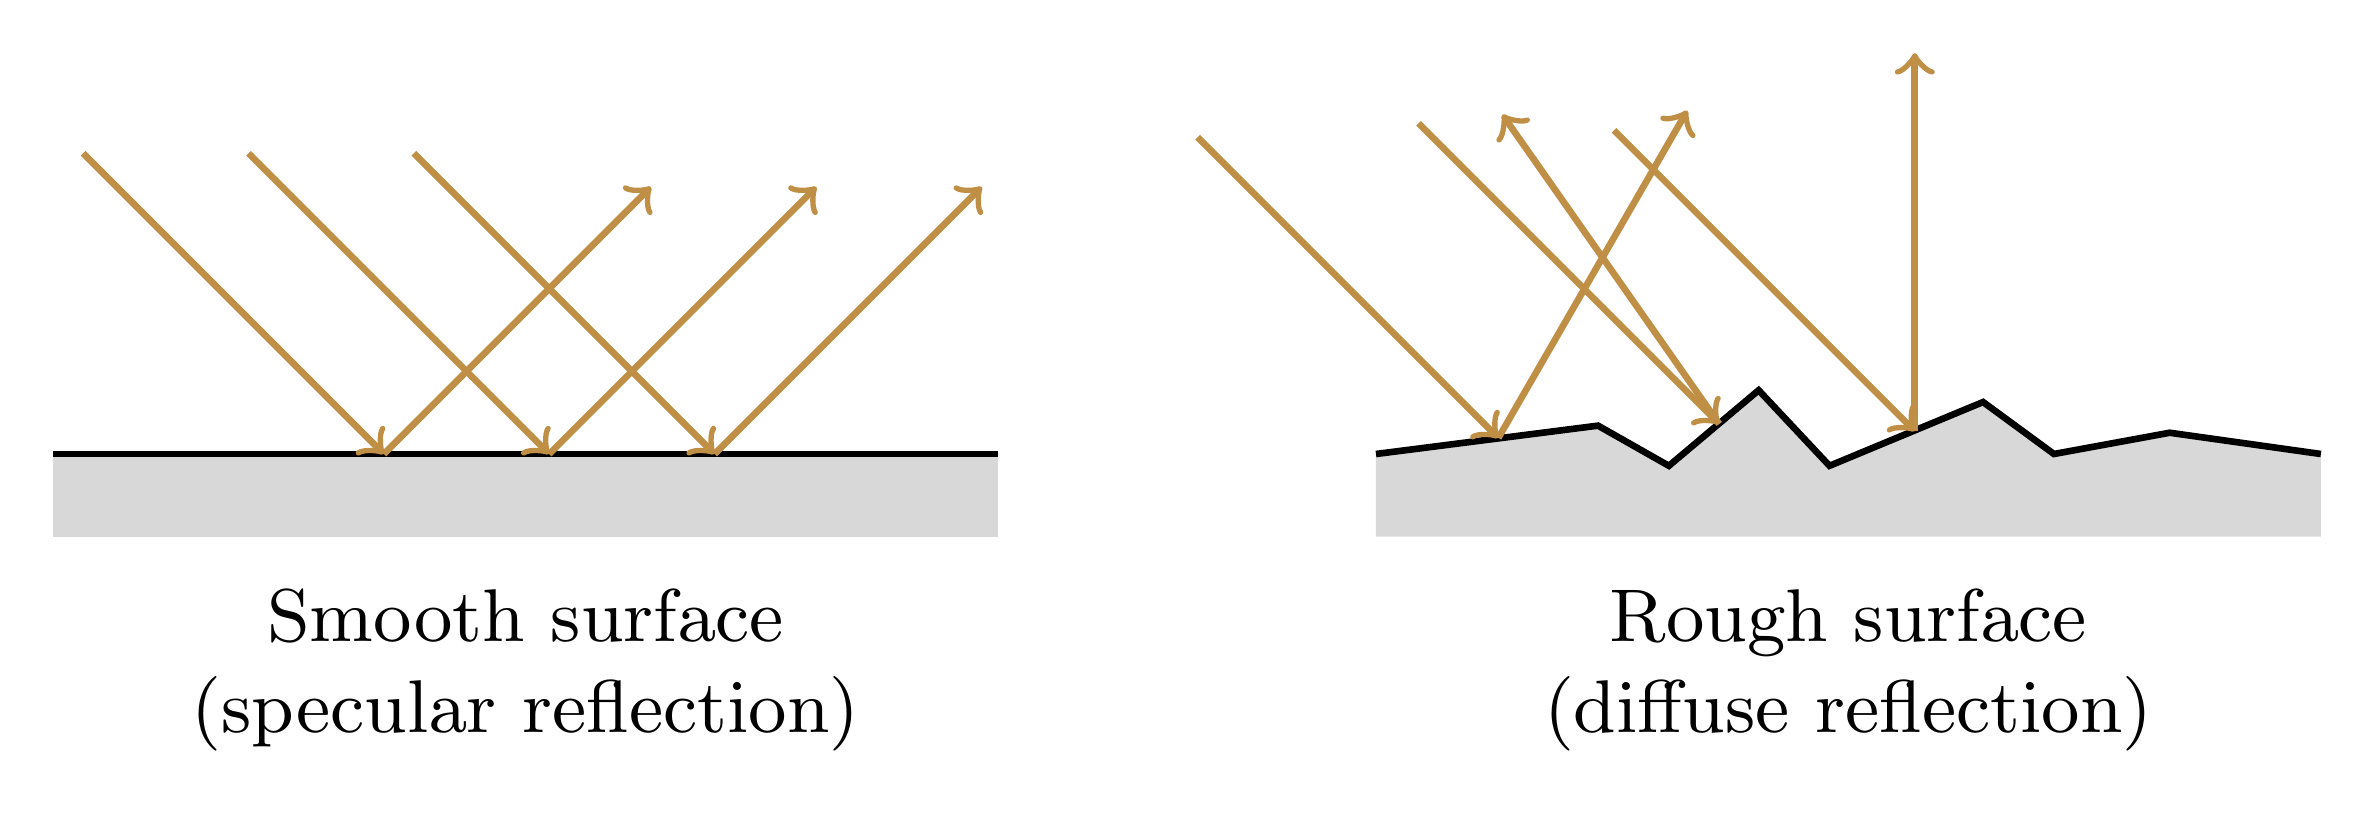
\includegraphics[width=0.72\textwidth]{refl_specular_diffuse.png}
    \caption{Parallel rays leave a smooth surface in one direction (specular reflection) and leave a rough surface in many directions (diffuse reflection).}
    \label{fig:refl-specular-diffuse}
\end{figure}

When a beam of light hits a mirror, it bounces off the mirror at the same
angle it approached from. That is, if it approaches nearly
perpendicular to the mirror, it departs nearly perpendicular to the
mirror. If it hits the mirror at a glancing angle, it departs at an
angle close to the mirror's surface. A good video to see this in action can be found here: \url{https://www.youtube.com/shorts/qA_VQZfTiUA}

\subsubsection{Law of Reflection}
\begin{figure}[H]
  \centering
  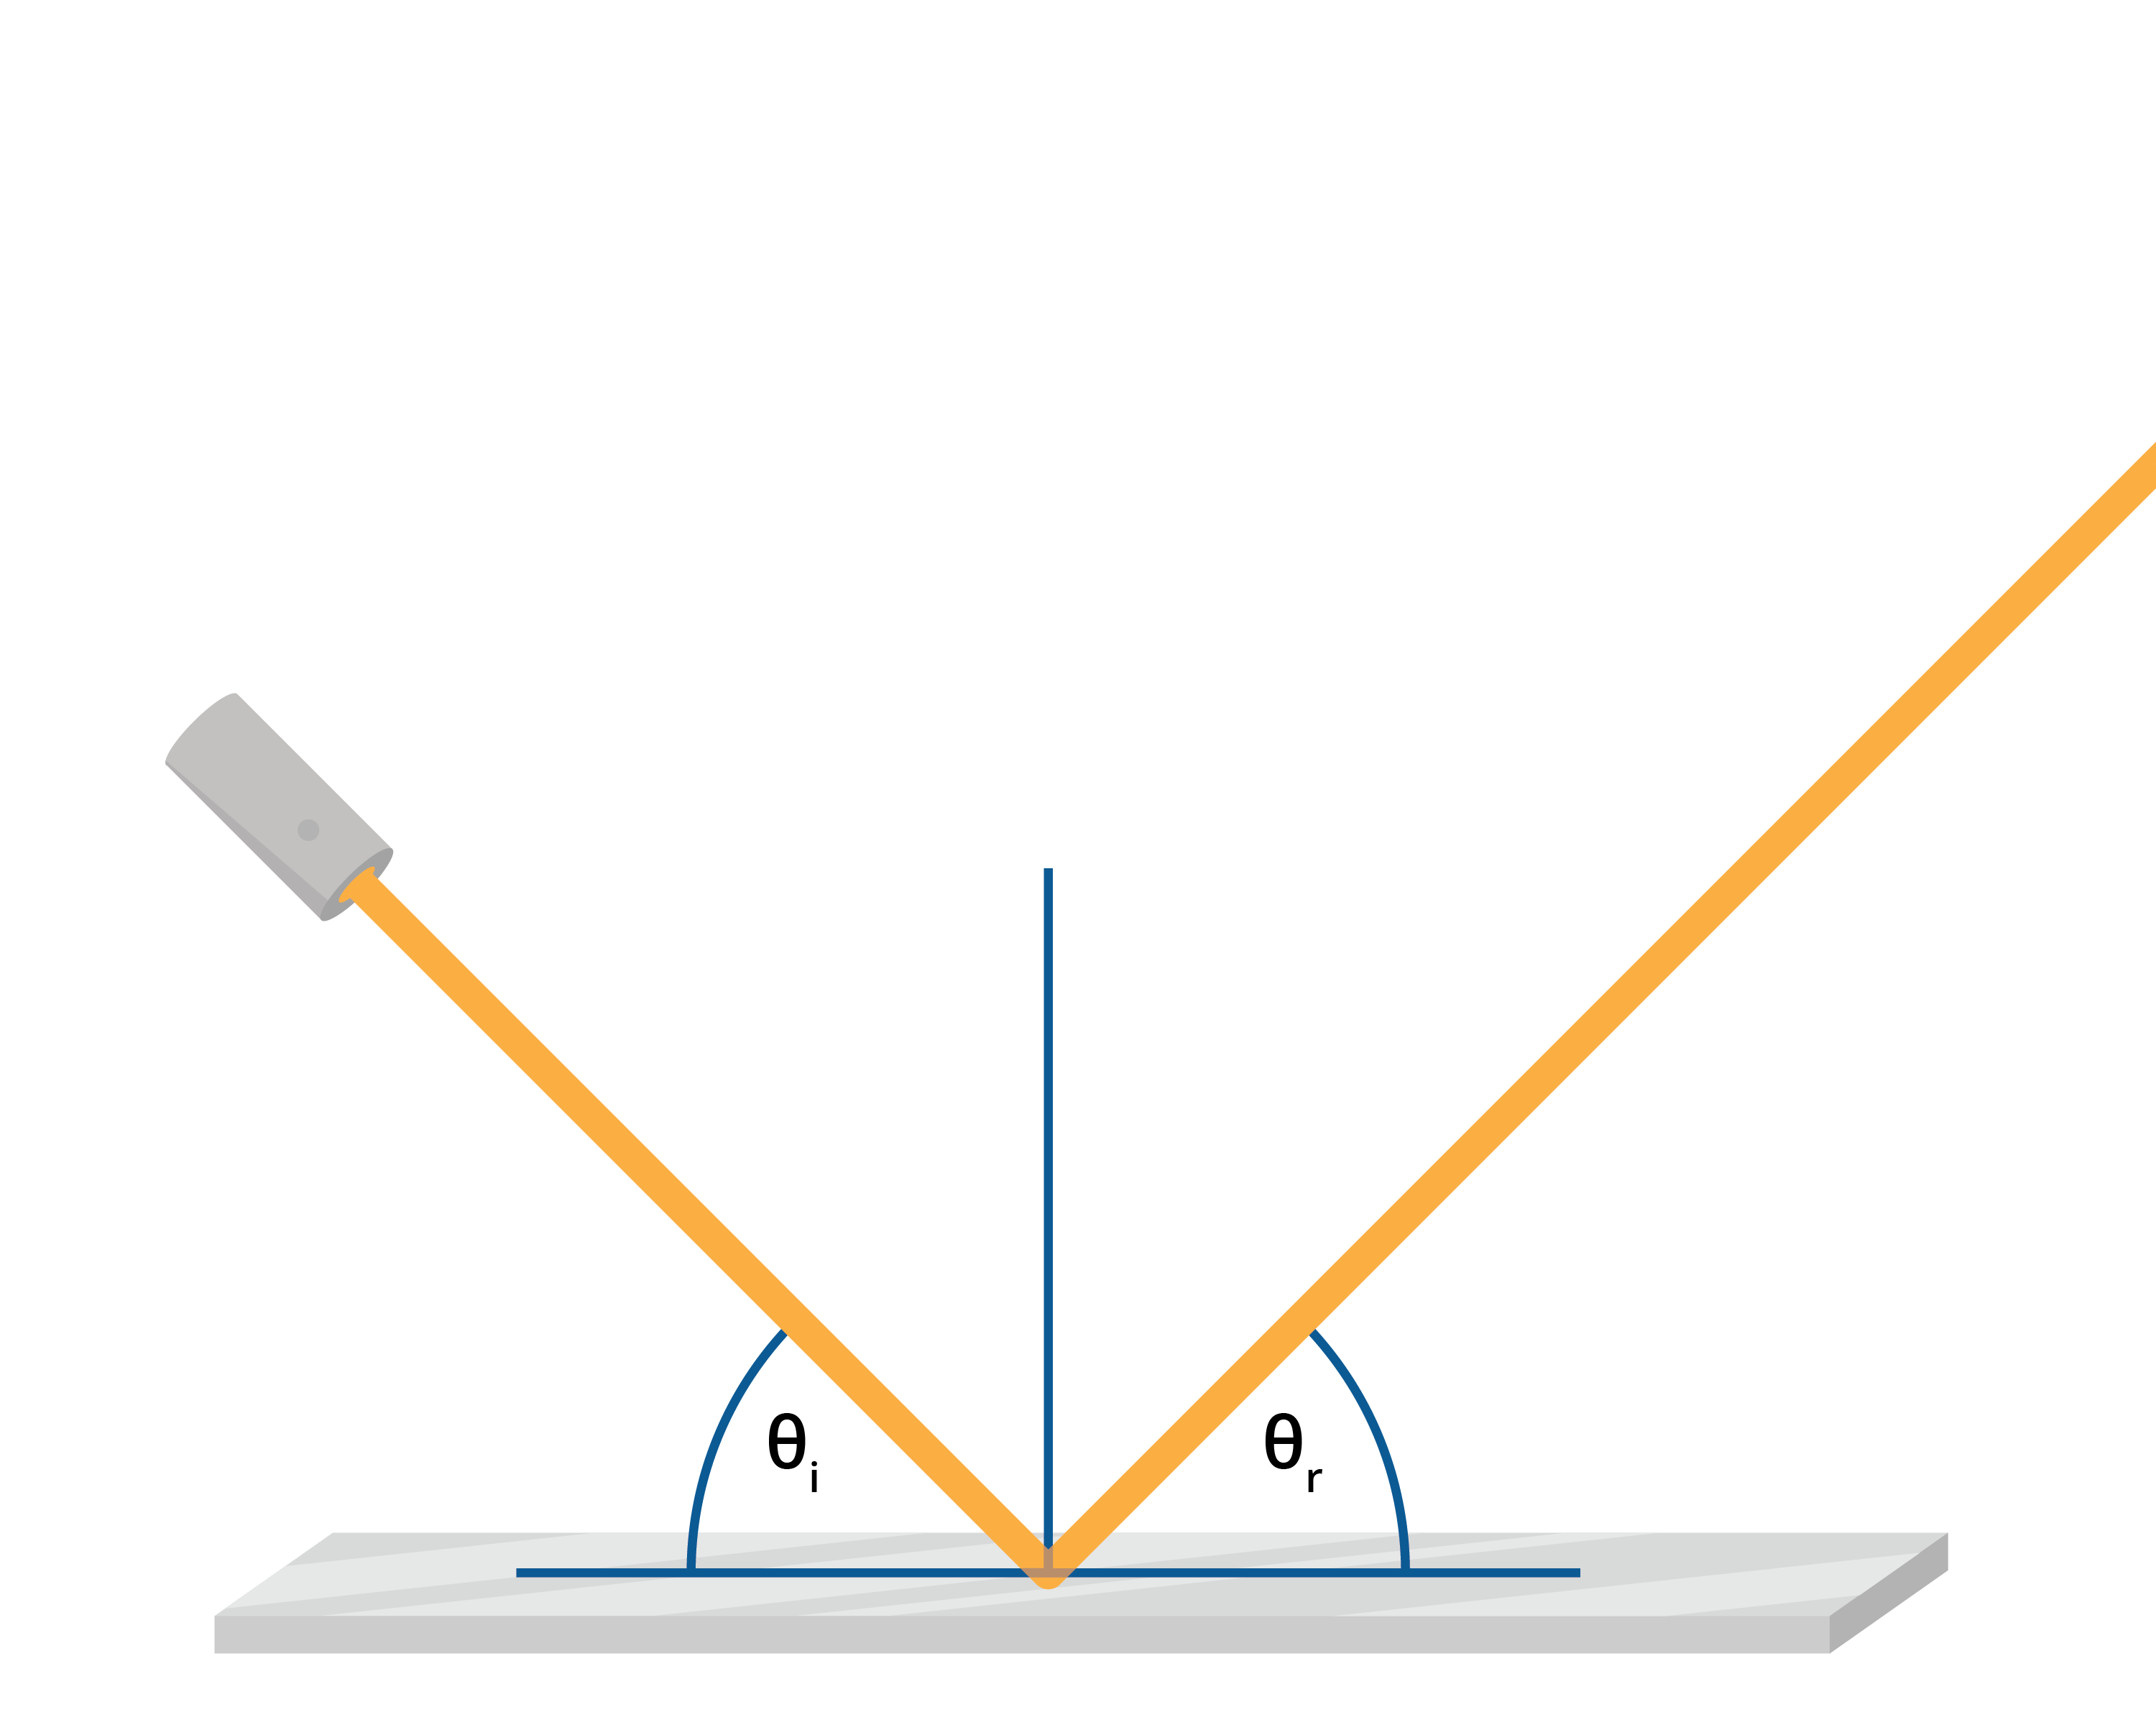
\includegraphics[width=1\textwidth]{reflection.png}
  \caption{The angle of \textit{incidence} is equal to the angle of \textit{reflection}.}
  \label{fig:lawOfReflectionImage}
\end{figure}

\begin{mdframed}[style=important, frametitle={Law of Reflection}]
  \index{reflection!Law of}
  The angle of incidence, denoted as $\theta_i$, is equal to
  the angle of reflection, denoted as $\theta_r$. This law can be
  mathematically expressed as:\index{reflection!law of}

  $$\theta_i = \theta_r$$

  where $\theta_i$ is the angle between the incident light ray and the
  normal to the surface, and $\theta_r$ is the angle between the
  reflected light ray and the normal.


  % \begin{figure}[H]
  %     \centering
  \begin{tikzpicture}[scale=5]
    \draw [black,thick](-0.7,0)--(0.7,0) node [midway, anchor=north]{Mirror};
    \draw [sdkblue,dashed,->] (0,0) -- (0,0.7) node [anchor=south]{Normal};
    \draw [sdkblue] (0,0.08) -- (0.08, 0.08) -- (0.08, 0);
    \draw [->](-0.5,0.8)--(-0.04,0.05);
    \draw [->](0,0)--(0.5,0.8);
    \draw [sdkblue,<->] (0, 0.3) arc (90:122:0.3)
    node [midway, anchor=south] {$\theta_i$};
    \draw [sdkblue,<->] (0, 0.3) arc (90:58:0.3)
    node [midway, anchor=south] {$\theta_r$};
  \end{tikzpicture}
  %     \caption{Diagram of Law of Reflection, where Normal is a perpendicular biceptor.}
  %     \label{fig:tikzLawOfReflection}
  % \end{figure}

\end{mdframed}

\begin{Exercise}[title={Law of Reflection}, label=law_of_reflection]

  You are standing 4 meters from a mirror hung on a wall. The bottom
  of the mirror is the same height as your chin, so you cannot see your
  whole body. You stick a piece of masking tape to your body.

  You walk forward until you are only 3 meters from the mirror, then
  put a piece of masking tape on your body at the new cut-off point. Is the new
  masking tape higher or lower on your body?

\end{Exercise}
\begin{Answer}[ref=law_of_reflection]

  Assuming the mirror is truly vertical and the floor is truly
  horizontal, the new cut off should be exactly the same as the old
  one: It should be below your chin the same amount that your eyes are
  above your chin.

  \textit{Illustration Here}

\end{Answer}


\subsection{Ellipses and Curved Mirrors}

Flat mirrors are common and useful, but things get more interesting
once you bend the mirrors. In this section, we are going to talk about
a few different kinds of curved mirrors.\index{circle!reflections in}

\subsubsection{The Reflective Properties of Circles and Spheres}

For example, if you were inside a circular room (a cylinder,
actually), you could imagine standing in the center and pointing a
flash light in any horizontal direction. The beam of light would
bounce right back to you. See Figure~\ref{fig:circlReflection}

\begin{figure}[H]
  \centering
  \begin{tikzpicture}[scale=1]
    \coordinate (a) at (0,0);
    \coordinate (b) at ({3 * cos(30)}, {3 * sin(30)});
    \draw [black, thick] (a) circle (3);
    \filldraw [sdkblue] (a) circle (2pt);
    \filldraw [sdkblue] (b) circle (2pt);
    \draw [sdkblue,<->] ({0.2 * cos(30)},{0.2 * sin(30)})--({2.8 * cos(30)},{2.8 * sin(30)});
  \end{tikzpicture}
  \caption{A circle would reflect back onto itself.}
  \label{fig:circlReflection}
\end{figure}

How do you know this?  Because the tangent line is always perpendicular to the radius to the point of tangency:
\begin{figure}[H]
  \centering
  \begin{tikzpicture}[scale=1.4]
    \coordinate (a) at (0,0);
    \coordinate (b) at ({3 * cos(30)}, {3 * sin(30)});
    \draw [black, thick] (3,0) arc (0:80:3);
    \filldraw [sdkblue] (a) circle (2pt);
    \filldraw [sdkblue] (b) circle (2pt);
    \draw [sdkblue,<->] ({0.2 * cos(30)},{0.2 * sin(30)})--({2.8 * cos(30)},{2.8 * sin(30)});
    \clip (-.1, -.1) rectangle (4,3);
    \draw [dashed] (0,{3 / sin(30)}) -- ({3 / cos(30)},0);
  \end{tikzpicture}
  \caption{The reflection on a circle uses a radius which hits a tangent line as a perpendicular bisector.}
  \label{fig:tangentCircle}
\end{figure}

You could create a spherical room with mirror walls. You would
create a platform in the center where you could stand, and if you
pointed your flashlight in any direction, its beam of light would
shine back at you.

\subsubsection{Ellipses and Ellipsoids}

Intuitively, you know what an ellipse is: an oval. However, the
ellipse is actually an oval with some special properties. This is a
good time to talk about those properties.\index{ellipse}

Mathematicians talk about a \newterm{standard} ellipse. A standard ellipse is
centered on the origin $(0,0)$ and its long axis is parallel with the
$x$-axis or the $y$-axis.

\begin{mdframed}[style=important, frametitle={Equation for a Standard Ellipse}]

  To be precise, a standard ellipse is the set of points $(x, y)$ that
  are solutions to the equation

  $$\frac{x^2}{a^2} + \frac{y^2}{b^2} = 1$$


  Note that $(a,0), (-a, 0), (0, b), (0,-b)$ are all part of the
  set. The complete set looks like this:

  % \begin{figure}[H]
  %     \centering
  \begin{tikzpicture}[scale=2]
    \draw [sdkblue, <->] (-2.5, 0)--(2.5, 0); \draw [sdkblue, <->] (0,
    -1.5)--(0, 1.5); \draw (0,0) ellipse (2 and 1); \filldraw [sdkblue]
    (-2, 0) circle (1pt) node [anchor=east] {$-a$}; \filldraw [sdkblue]
    (2, 0) circle (1pt) node [anchor=west] {$a$}; \filldraw [sdkblue]
    (0, -1) circle (1pt) node [anchor=north] {$-b$}; \filldraw [sdkblue]
    (0, 1) circle (1pt) node [anchor=south] {$b$};
  \end{tikzpicture}
  %     \caption{The points on an ellipse.}
  %     \label{fig:ellipsePoints}
  % \end{figure}

  The area contained inside this ellipse is given by

  $$A = \pi a b$$


\end{mdframed}


We can now talk about two special points: the \newterm{foci}. Each
focal point is on the long axis of the ellipse. Let us assume for a
moment that $a > b$. (Everything works the same if $b > a$, but it
gets confusing if we try to deal with both cases simultaneously.)\index{ellipse!focus points}

If $p$ is a point on the ellipse, the distance from $p$ to focal point 1
plus the distance from $p$ to focal point 2 is always $2a$.
\begin{figure}[H]
  \centering
  \begin{tikzpicture}[scale=2]
    \coordinate (p) at (0.7, 0.93674969975976);
    \coordinate (f1) at (-1.732050807568877, 0);
    \coordinate (f2) at (1.732050807568877, 0);
    \draw [sdkblue, <->] (-2.5, 0)--(2.5, 0);
    \draw [sdkblue, <->] (0, -1.5)--(0, 1.5);
    \draw (0,0) ellipse (2 and 1);
    \filldraw [sdkblue] (-2, 0) circle (1pt) node [anchor=east] {$-a$};
    \filldraw [sdkblue] (2, 0) circle (1pt) node [anchor=west] {$a$};
    \filldraw [sdkblue] (0, -1) circle (1pt) node [anchor=north] {$-b$};
    \filldraw [sdkblue] (0, 1) circle (1pt) node [anchor=south] {$b$};
    \filldraw (p) circle (1pt) node [anchor=south] {$p$};
    \filldraw (f1) circle (1pt) node [anchor=north] {$f_1$};
    \filldraw (f2) circle (1pt) node [anchor=north] {$f_2$};
    \draw [dashed] (f1) -- (p) node [midway, anchor=south] {$d$};
    \draw [dashed] (f2) -- (p) node [midway, anchor=north] {$2a - d$};
  \end{tikzpicture}
  \caption{The both foci and point p forms a triangle with legs $2a-d$ or $d$.}
  \label{fig:pointPTriangle}
\end{figure}

How do we find the foci? We know they are on the long axis and that
they are symmetrical across the short axis. All we need to know is how
far are they from the short axis.

\begin{mdframed}[style=important, frametitle={Distance from Center to the Foci}]

  If you have an ellipse with a long axis that extends $a$ from the center,
  and a short axis that extends $b$ from the center, the foci
  lie on the long axis and are $c$ from the center. Where

  $$c = \sqrt{a^2 - b^2}$$

\end{mdframed}

\begin{Exercise}[title={Foci of an ellipse}, label=ellipse_foci]

  You need to draw an ellipse that is 12 cm long and 7 cm wide. You
  have a string, two pushpins, a ruler, and a pencil. Using the ruler,
  you draw two perpendicular axes.

  You will stick one pin at each focal point. Each end of the string
  will be tied to a push pin. Using the pencil to keep the string taut, you will draw
  an ellipse.

  \begin{tikzpicture}[scale=.2]
    \coordinate (p) at (-3, 6.77772085586298);
    \coordinate (f1) at (-9.746794344808964, 0);
    \coordinate (f2) at (9.746794344808964, 0);
    \draw [sdkblue, <-] (-14, 0)--(12, 0);
    \draw [sdkblue, <-] (0, -9)--(0, 7);
    \draw (0,0) ellipse (12 and 7);
    \filldraw [sdkblue] (-12, 0) circle (4pt);
    \filldraw [sdkblue] (12, 0) circle (4pt) node [anchor=west] {12 cm};
    \filldraw [sdkblue] (0, -7) circle (4pt);
    \filldraw [sdkblue] (0, 7) circle (4pt) node [anchor=south] {7 cm};
    \filldraw (p) circle (4pt) ;
    \filldraw (f1) circle (4pt);
    \filldraw (f2) circle (4pt);
    \draw [dashed] (f1) -- (p);
    \draw [dashed] (f2) -- (p);
  \end{tikzpicture}

  How far from the short axis are the pushpins placed?

  How long is the string between them?

\end{Exercise}
\begin{Answer}[ref=ellipse_foci]

  The length of the string is easy: $2 \times 12 = 24$ cm.

  The distance from the center to the focal point is $\sqrt{12^2 - 7^2} \approx 6.78$ cm.

  \begin{tikzpicture}[scale=.2]
    \coordinate (p) at (-3, 6.77772085586298);
    \coordinate (f1) at (-9.746794344808964, 0);
    \coordinate (f2) at (9.746794344808964, 0);
    \draw [sdkblue, <-] (-14, 0)--(12, 0);
    \draw [sdkblue, <-] (0, -9)--(0, 7);
    \draw (0,0) ellipse (12 and 7);
    \filldraw [sdkblue] (-12, 0) circle (4pt);
    \filldraw [sdkblue] (12, 0) circle (4pt) node [anchor=west] {12 cm};
    \filldraw [sdkblue] (0, -7) circle (4pt);
    \filldraw [sdkblue] (0, 7) circle (4pt) node [anchor=south] {7 cm};
    \filldraw (p) circle (4pt) ;
    \filldraw (f1) circle (4pt);
    \filldraw (f2) circle (4pt);
    \draw [dashed] (f1) -- (p) node [midway, anchor=south] {$d$};
    \draw [dashed] (f2) -- (p) node [midway, anchor=south] {$24 - d$};
    \draw (6,0) node [anchor=north] {6.78 cm};
  \end{tikzpicture}

\end{Answer}

\subsubsection{The Reflective Property of Ellipses}

Here is something else that is wonderful about an ellipse: Pick any
point $p$ on the ellipse. Draw a line from $p$ to each focal point.
Draw the line tangent to the ellipse at $p$. You will see that the angle between
the tangent and the line to focal point 1 is equal to the angle between the
tangent and the line to focal point 2. See Figure~\ref{fig:reflectiveEllipse}
\begin{figure}[H]
  \centering
  \begin{tikzpicture}[scale=2]
    \coordinate (p) at (0.7, 0.93674969975976);
    \coordinate (f1) at (-1.732050807568877, 0);
    \coordinate (f2) at (1.732050807568877, 0);
    \clip (-2.5, -.4) rectangle (5.5,2);
    \draw [sdkblue] (-2.1, 0)--(2.1, 0);
    \draw [sdkblue] (0, -1.1)--(0, 1.1);
    \draw (0,0) ellipse (2 and 1);
    \filldraw (p) circle (1pt) node [anchor=south] {$p$};
    \filldraw (f1) circle (1pt) node [anchor=north] {$f_1$};
    \filldraw (f2) circle (1pt) node [anchor=north] {$f_2$};
    \draw [sdkblue] (f1) -- (p);
    \draw [sdkblue] (f2) -- (p);
    \coordinate (t1) at (-0.2829937278, 1.120388832);
    \coordinate (t2) at (1.682993728, 0.7531105671);
    \draw [dashed, thick]  (t1)--(t2);
    \draw [sdkblue, <->] (t1) arc (169.4181988:201.0651201:1)
    node [midway, anchor=east] {$\theta$};
    \draw [sdkblue, <->] (t2) arc (-10.5818012:-42.22872252:1)
    node [midway, anchor=east] {$\theta$};
  \end{tikzpicture}
  \caption{Reflective Property of Ellipses.}
  \label{fig:reflectiveEllipse}
\end{figure}

This is known as ``The Reflective Property of Ellipses''.
\index{ellipse!reflective property of}
Imagine you and your friend Fred are at an ellipse-shaped skating rink, and the
edge of the rink is mirrored. You sit at one focal point and your friend
sits at the other. If you point a flashlight at the mirror (in any
direction!), the beam will bounce off the wall and head directly for
Fred.

If Fred ducks out of the way, the beam will bounce again and
head back to you.
\begin{figure}[H]
  \centering
  \begin{tikzpicture}[scale=4]
    \coordinate (p) at (0.7, 0.93674969975976);
    \coordinate (p2) at (1.95763,-0.204758);
    \coordinate (f1) at (-1.732050807568877, 0);
    \coordinate (f2) at (1.732050807568877, 0);
    \draw (0,0) ellipse (2 and 1);
    \filldraw [sdkblue] (p) circle (0.5pt);
    \filldraw [sdkblue] (p2) circle (0.5pt);
    \filldraw (f1) circle (1pt) node [anchor=north] {You};
    \filldraw (f2) circle (1pt) node [anchor=north] {Fred};
    \draw [sdkblue, ->] (f1) -- (p);
    \draw [sdkblue, ->] (p) -- (p2);
    \draw [sdkblue, ->] (p2) -- (f1);
    \coordinate (b1) at (0.6081804337,0.4452528358);
    \coordinate (b2) at (1.219613217,0.1039995564);
    \draw [dashed] (p)--(b1);
    \draw [dashed] (p2)--(b2);
    \coordinate (t1) at (0.1102037633, 1.046933179);
    \coordinate (t2) at (1.289796237, 0.8265662202);
    \draw [dashed, thick]  (t1)--(t2);
    \draw [dashed, thick] (1.764656527,-0.6660184891) -- (2.150603473,0.2565024891);
    \draw [sdkblue, <->] (b1) arc (-100.5818012:-42.22872252:0.5)
    node [midway, anchor=south] {$\theta_1$};
    \draw [sdkblue, <->] (b1) arc (-100.5818012:-158.9348799:0.5)
    node [midway, anchor=south] {$\theta_1$};
    \draw [sdkblue, <->] (b2) arc (157.2974596:137.7712775:0.8)
    node [midway, anchor=west] {$\theta_2$};
    \draw [sdkblue, <->] (b2) arc (157.2974596:176.8236417:0.8)
    node [midway, anchor=west] {$\theta_2$};
  \end{tikzpicture}
  \caption{Your laser intersects Fred.}
  \label{fig:laserFred}
\end{figure}

This will work for sound as well. If you whisper while on the focal point, Fred
(at the other focal point) will hear you surprisingly well, because all
the soundwaves that hit the wall will bounce (just like the light)
straight at Fred.

\subsubsection{Elliptical Orbits}

One more fun fact about ellipses: We often imagine the planets
traveling in circular orbits with the sun at the center --- they
actually travel in elliptical orbits, with the sun as one of the focal
points.\index{elliptical!orbit}

The Earth is closest to the sun around January 3rd: 147 million km.

The Earth is farthest from the sun around July 3rd: 152 million km.

(Note that these dates are not the same as the solstices: The southern
hemisphere is tilted the most toward the sun around December 21 and
tilted most away around June 21.)

\subsubsection{Ellipsoids}

Just as we can pull the ideas of a circle into three dimensions to
make a sphere, we can extend the ideas of the ellipse into three
dimensions to talk about ellipsoids. Ellipsoids are like blimps.\index{ellipsoid}

The standard ellipsoids are centered at the origin and aligned with the three axes.

\begin{mdframed}[style=important, frametitle={Equation for a Standard Ellipsoid}]

  To be precise, a standard ellipsoid is the set of points $(x, y, z)$ that
  satisfy the equation

  $$\frac{x^2}{a^2} + \frac{y^2}{b^2} + \frac{z^2}{c^2}= 1$$


  Note that $(a,0,0), (0, b,0), (0,0,c)$ are all part of the
  set. The complete set looks like this:
  \begin{center}
    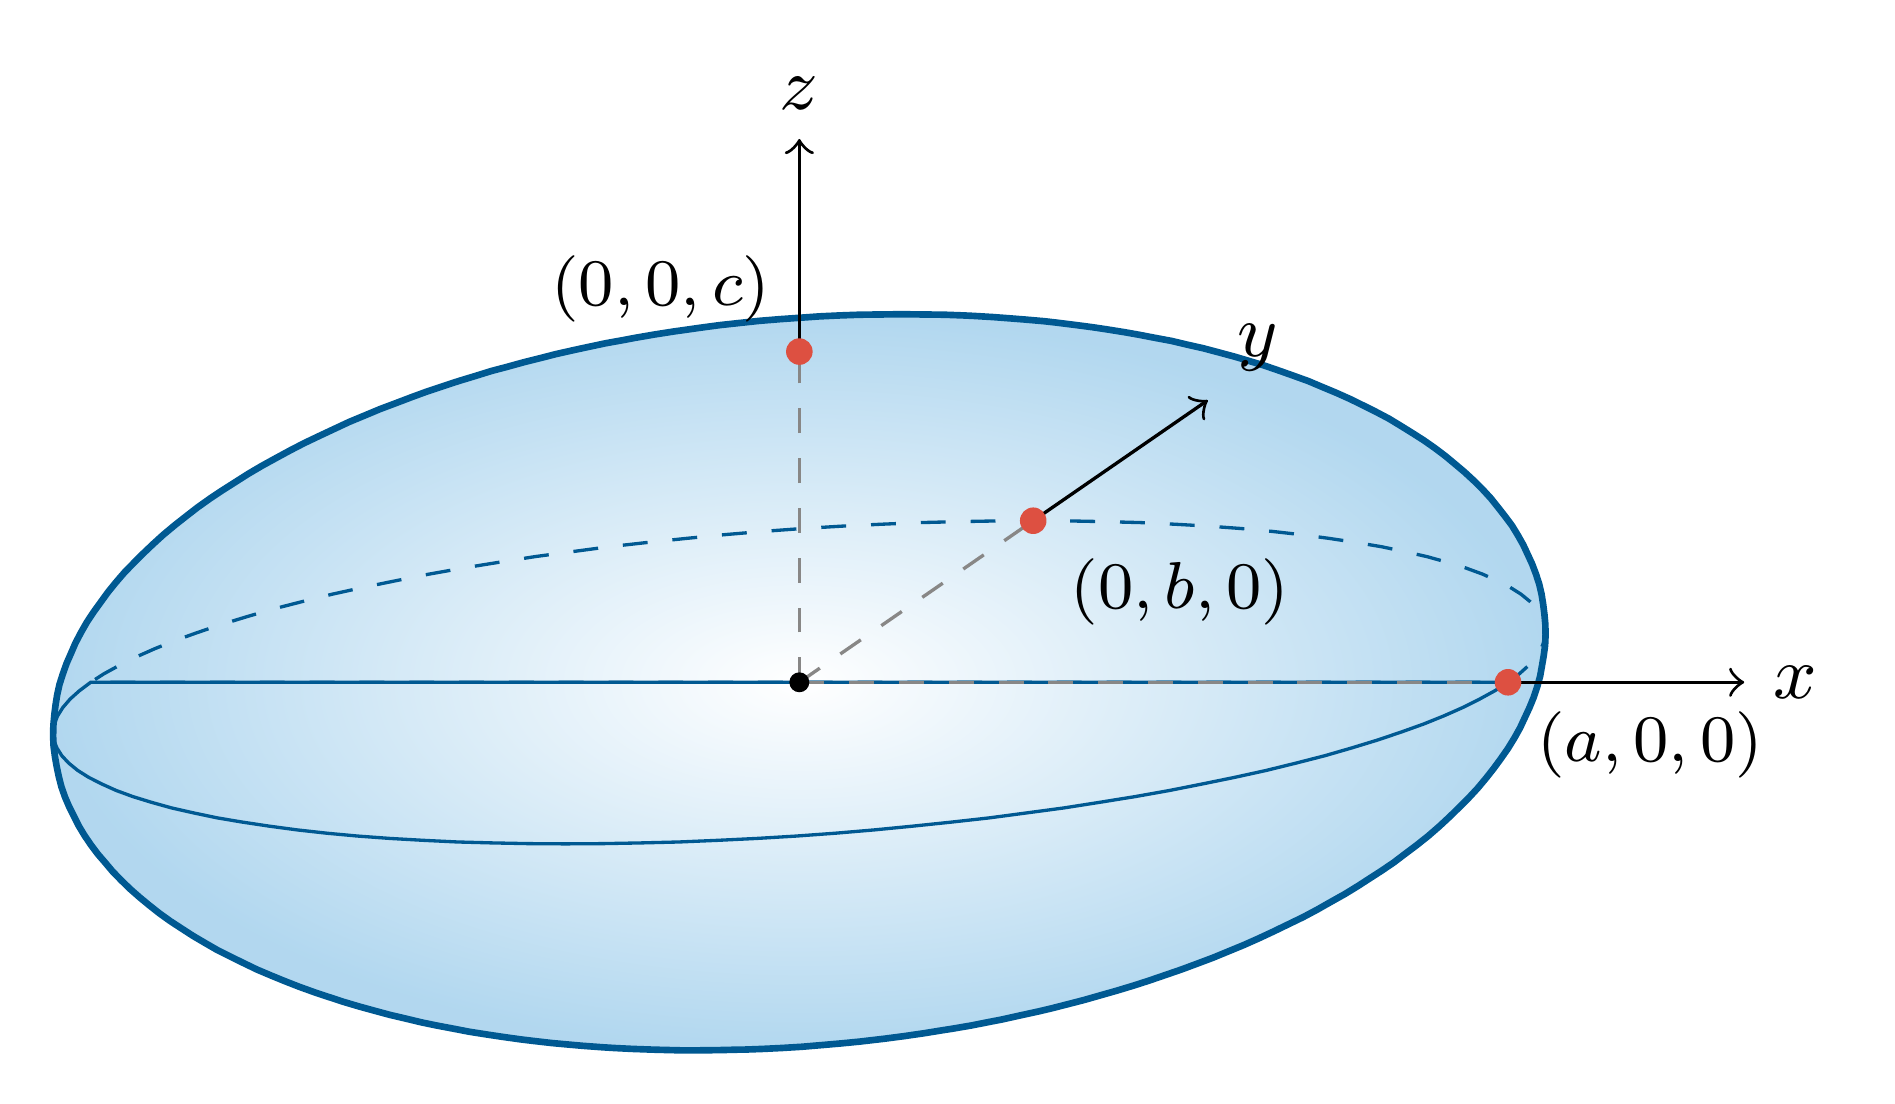
\includegraphics[width=0.5\linewidth]{refl_ellipsoid.png}
  \end{center}

  The volume bounded by this ellipsoid is

  $$V = \frac{4}{3} \pi a b c$$


\end{mdframed}

Of course, $a$, $b$, and $c$ can be any positive number, but in the
real world, we find ourselves working regularly with ellipsoids where two
of the numbers are the same.

\subsubsection{Oblate Spheroid}

If two axes have the same length and one is shorter, you get something
that looks like a sphere compressed in one direction --- like a
pumpkin. These are called \newterm{oblate spheroids}.\index{oblate spheroid}

The Earth is actually an oblate spheroid; the axis that goes through
the north and south pole is shorter than the axes that pass through
the equator. How much shorter? Just a little, relatively speaking. The equator is 6,378 km
from the center of the Earth; the north pole is 21 km closer.\index{earth!shape of}

\subsubsection{Prolate Spheroid}

If two axes have the same length and one is longer, you get something
that looks like a sphere stretched in one direction --- like a rugby
ball. It is called a \newterm{prolate spheroid}.\index{prolate spheroid}

Like an ellipse, prolate spheroids have two focal points.

\begin{mdframed}[style=important, frametitle={Focal Points of a Prolate Spheroid}]

  If the long axis has a radial length of $a$ and the two shorter axes
  have radial length $b$, then the focal points are on the long axis. The distance from the center to the focal point is given by

  $$c = \sqrt{a^2 - b^2}$$

  For any point $p$ on the prolate spheroid, the sum of the distances
  from $p$ to the focus points will always be $2a$.

  It has the reflective property: A photon shot in any direction
  from one focal point will bounce off the wall and head directly at the other.

\end{mdframed}

\begin{Exercise}[title={Volume of a Rugby Ball}, label=rugby_ball]

  Some jokesters once thought it would be fun to make something that looked like a rugby ball, but made out of lead.

  A rugby ball is about 30 cm long and has a circumference of 60 cm at
  its midpoint. A cubic centimeter of lead has a mass of 11.34 grams.

  How much would a solid (not hollow) lead rugby ball weigh?

\end{Exercise}
\begin{Answer}[ref=rugby_ball]

  We need the distance from the center out to each of the three axes. We know that $a = \left(\frac{1}{2} \right) 30 = 15$ cm.

  We can calculate the $b$ and $c$ (which are equal) using the circumference given: $2b\pi = 60$, so $c = b \approx 9.55$ cm.

  The volume, then is

  $$V = \frac{4}{3} \pi (15)(9.55)(9.55) \approx 5,730 \text{ cubic centimeters }$$

  The mass would be $5,730 \times 11.34 = 64,973$ grams or about 65 kg.
\end{Answer}

\subsubsection{Parabolas and Parabolic Reflectors}

You are familiar with quadratic functions:

$$y = a x^2 + b x + c$$

If $a$ is not zero, the graph of a quadratic is a curved line called a
\newterm{parabola}\index{parabola}. The first parabola that most mathematicians think of is the graph of $y = x^2$:

\begin{tikzpicture}
  \draw[sdkblue,<->] (-2.0, 0) -- (2.0, 0) node[right] {$x$};
  \draw[sdkblue,<->] (0, -1) -- (0, 5) node[above] {$y$};
  \draw[domain=-1.9:1.9,samples=300,variable=\x,<->]  plot (\x,{\x*\x});
  \draw (1.1, 1) node [anchor=west] {$y = x^2$};
\end{tikzpicture}

\begin{figure}[H]
    \centering
    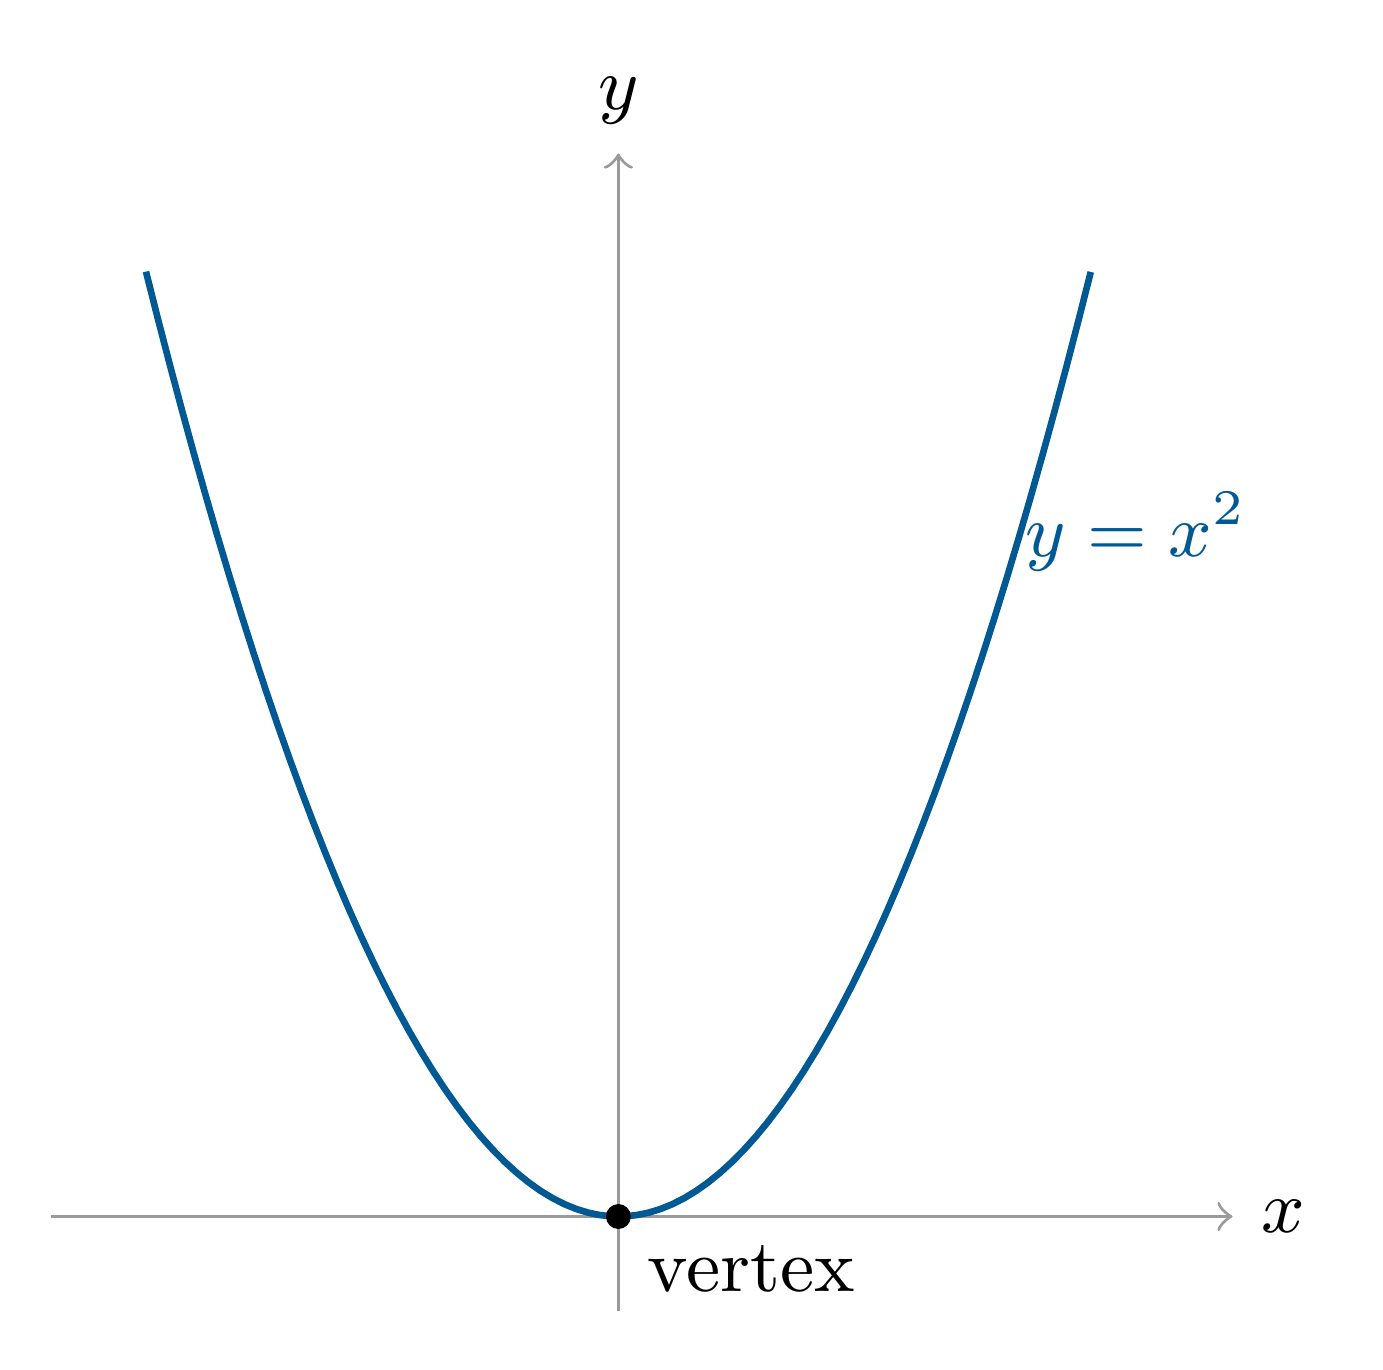
\includegraphics[width=0.36\textwidth]{refl_parabola_basic.png}
    \caption{The graph of $y = x^2$ is a parabola with its vertex at the origin.}
    \label{fig:refl-parabola-basic}
\end{figure}
Every parabola has a \newterm{focus} and a \newterm{directrix}. The
focus is a point on the parabola's axis of symmetry. The directrix is
a line perpendicular to the axis of symmetry. Every point on the
parabola is equal distance from the focus and the directrix.

For the graph of $y = x^2$, the focus is the point $(0, \frac{1}{4})$. The directrix is the line $y = -\frac{1}{4}$:

\begin{figure}[H]
    \centering
    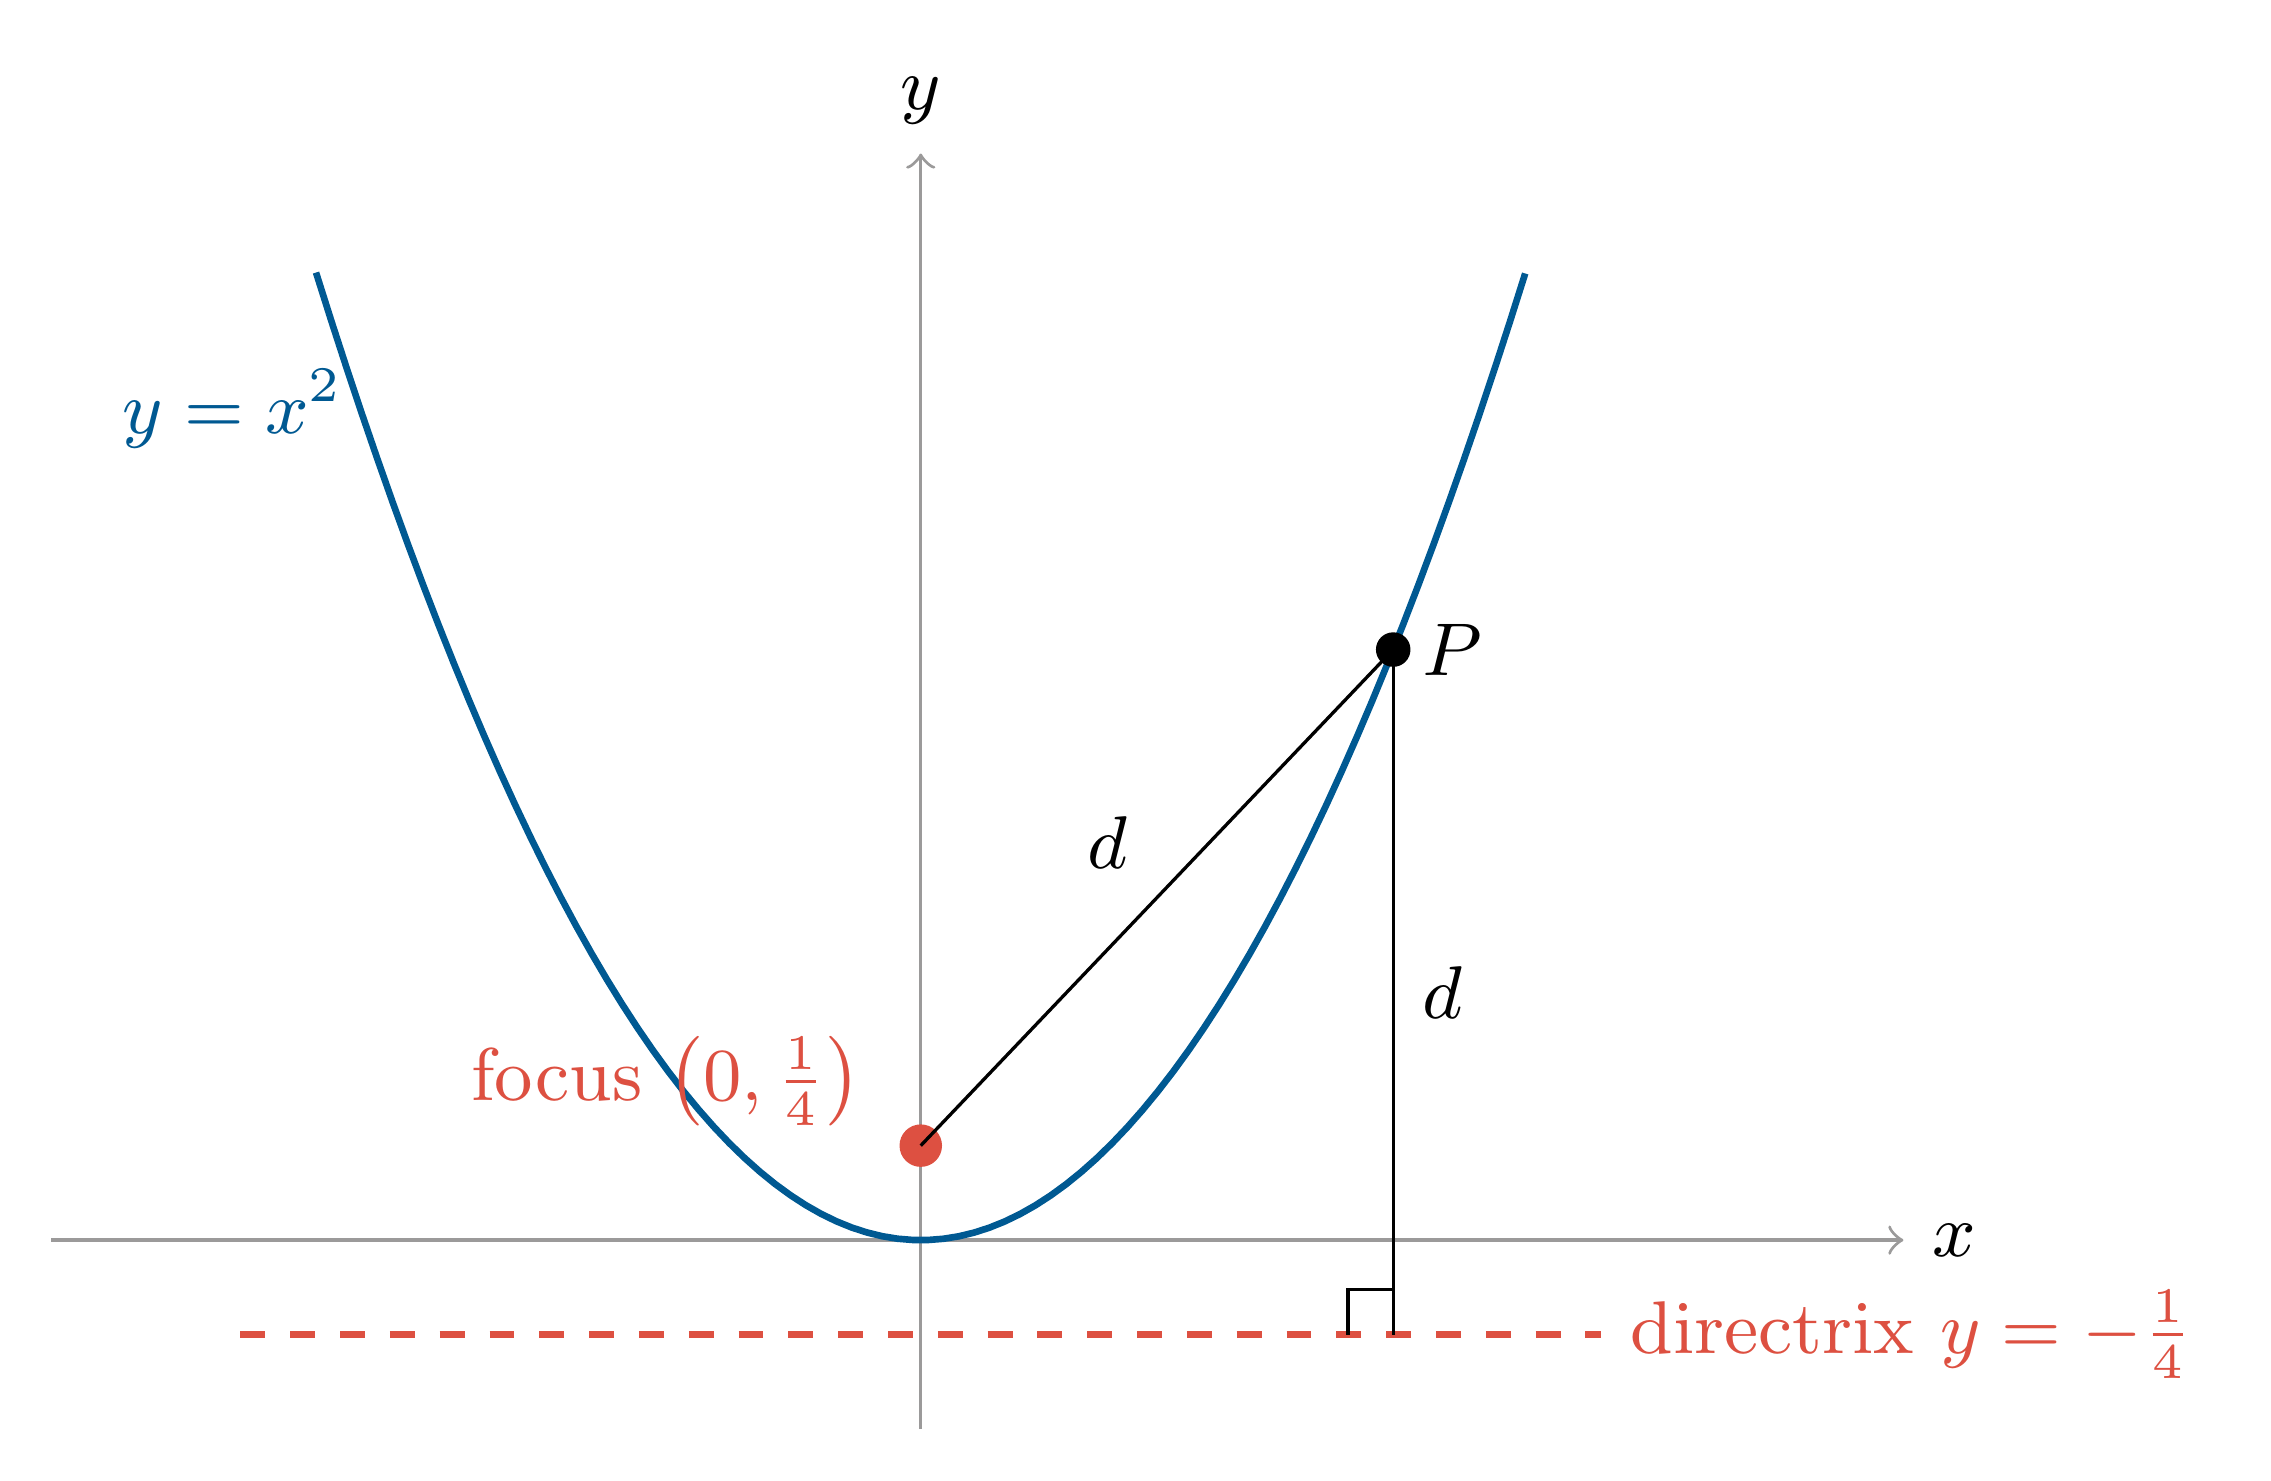
\includegraphics[width=0.58\textwidth]{refl_focus_directrix.png}
    \caption{Every point $P$ on $y = x^2$ is the same distance $d$ from the focus $\left(0, \frac{1}{4}\right)$ and from the directrix $y = -\frac{1}{4}$.}
    \label{fig:refl-focus-directrix}
\end{figure}


For example, the point $(1,1)$ is on this parabola. It is 5/4 from the
directrix. How far is it from the focus?  1 horizontally and 3/4 vertically.

$$\sqrt{1^2 + \left( \frac{3}{4} \right)^2} = \frac{5}{4}$$

Thus, we have confirmed that $(1,1)$ is equal distances from the focus
and the directrix.

When we think about a parabola and its properties, we usually rotate
and translate it to be symmetric around the $y$-axis, flip it so that
it is low in the middle and rising on both sides, and push it up or
down until the low point is on the $x$-axis.

Then, they can all be written:

$$y = \frac{a}{4} x^2$$

where $a > 0$. If $a$ is small, the parabola opens wider.

\begin{figure}[H]
    \centering
    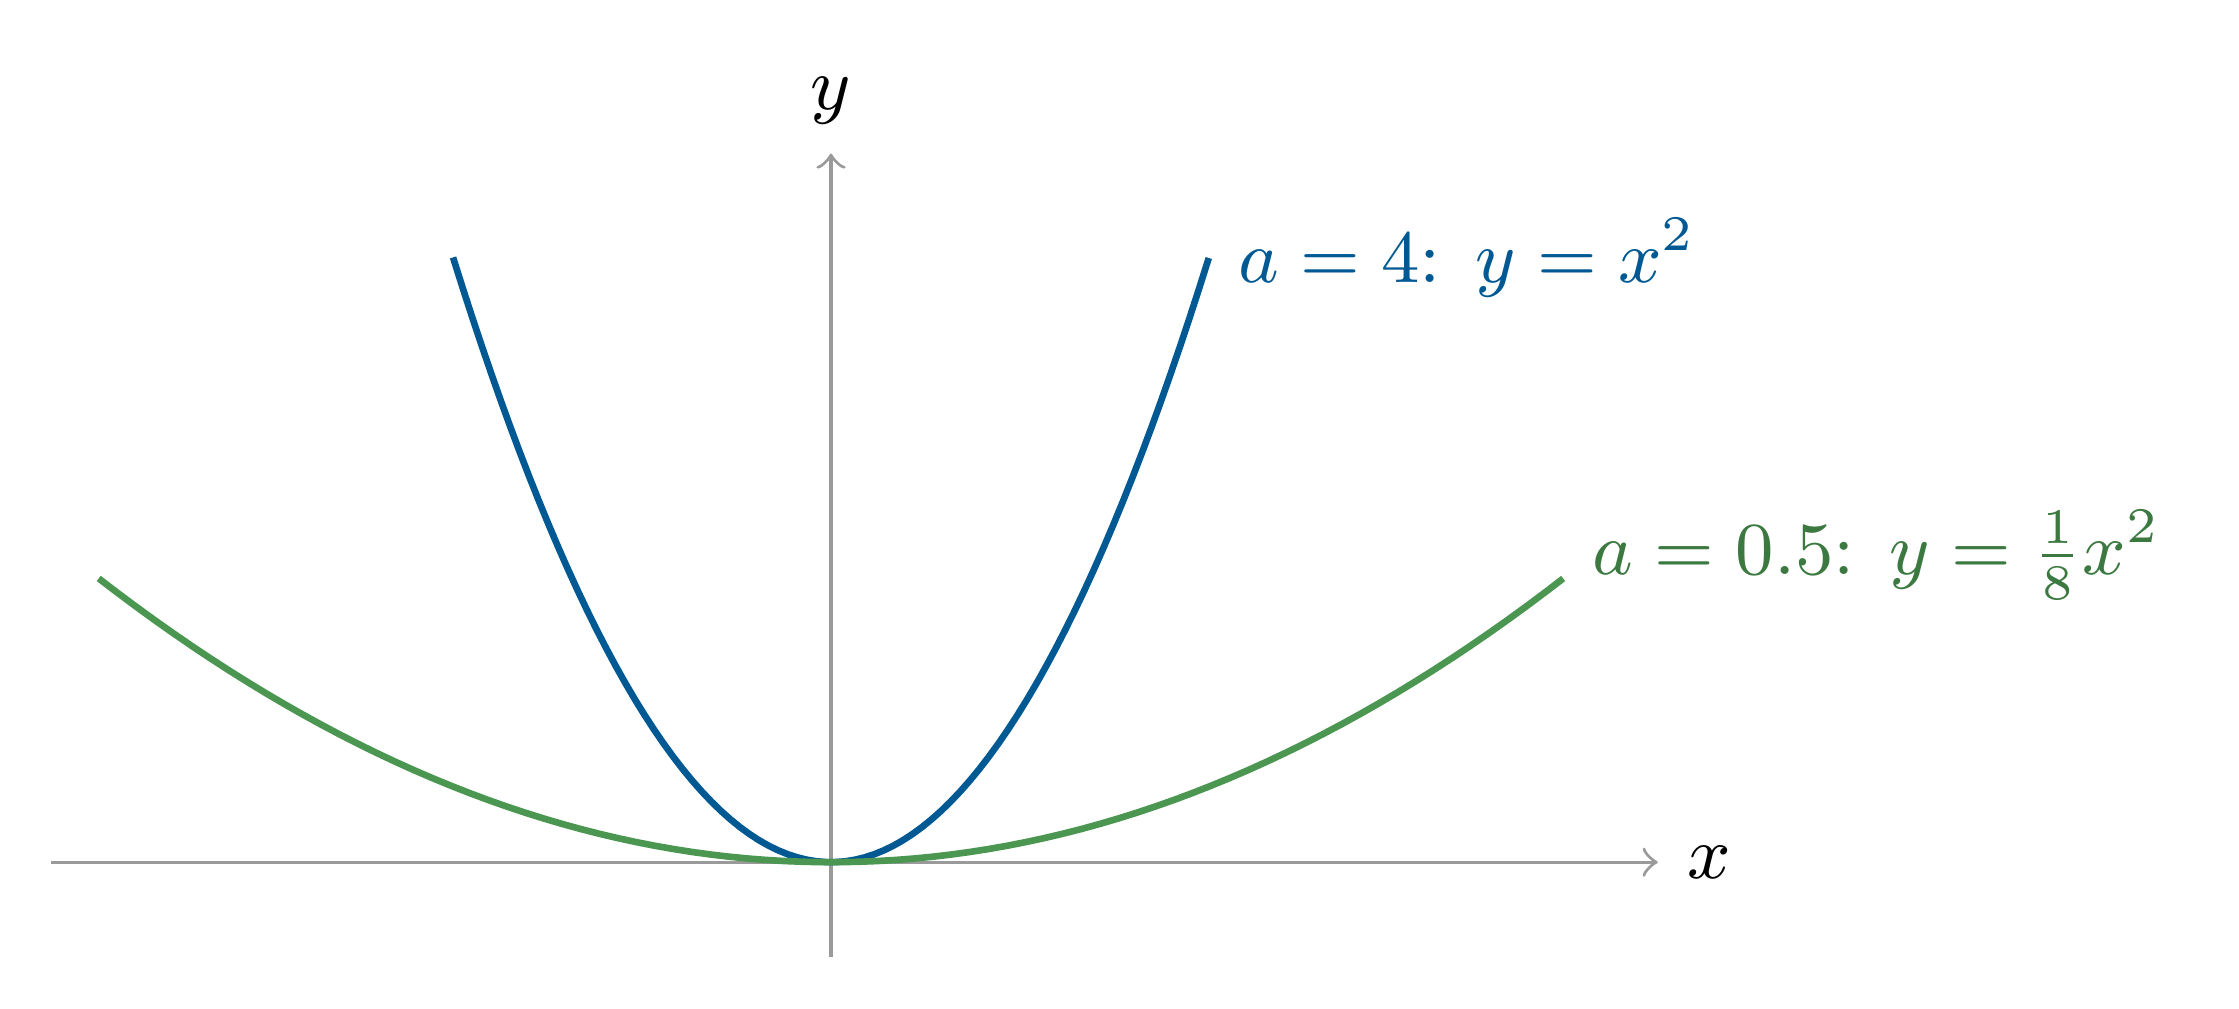
\includegraphics[width=0.57\textwidth]{refl_parabola_widths.png}
    \caption{A smaller value of $a$ gives a wider parabola.}
    \label{fig:refl-parabola-widths}
\end{figure}

The focus is at $(0, \frac{1}{a})$ and the directrix is the line $y = -\frac{1}{a}$.

\begin{figure}[H]
    \centering
    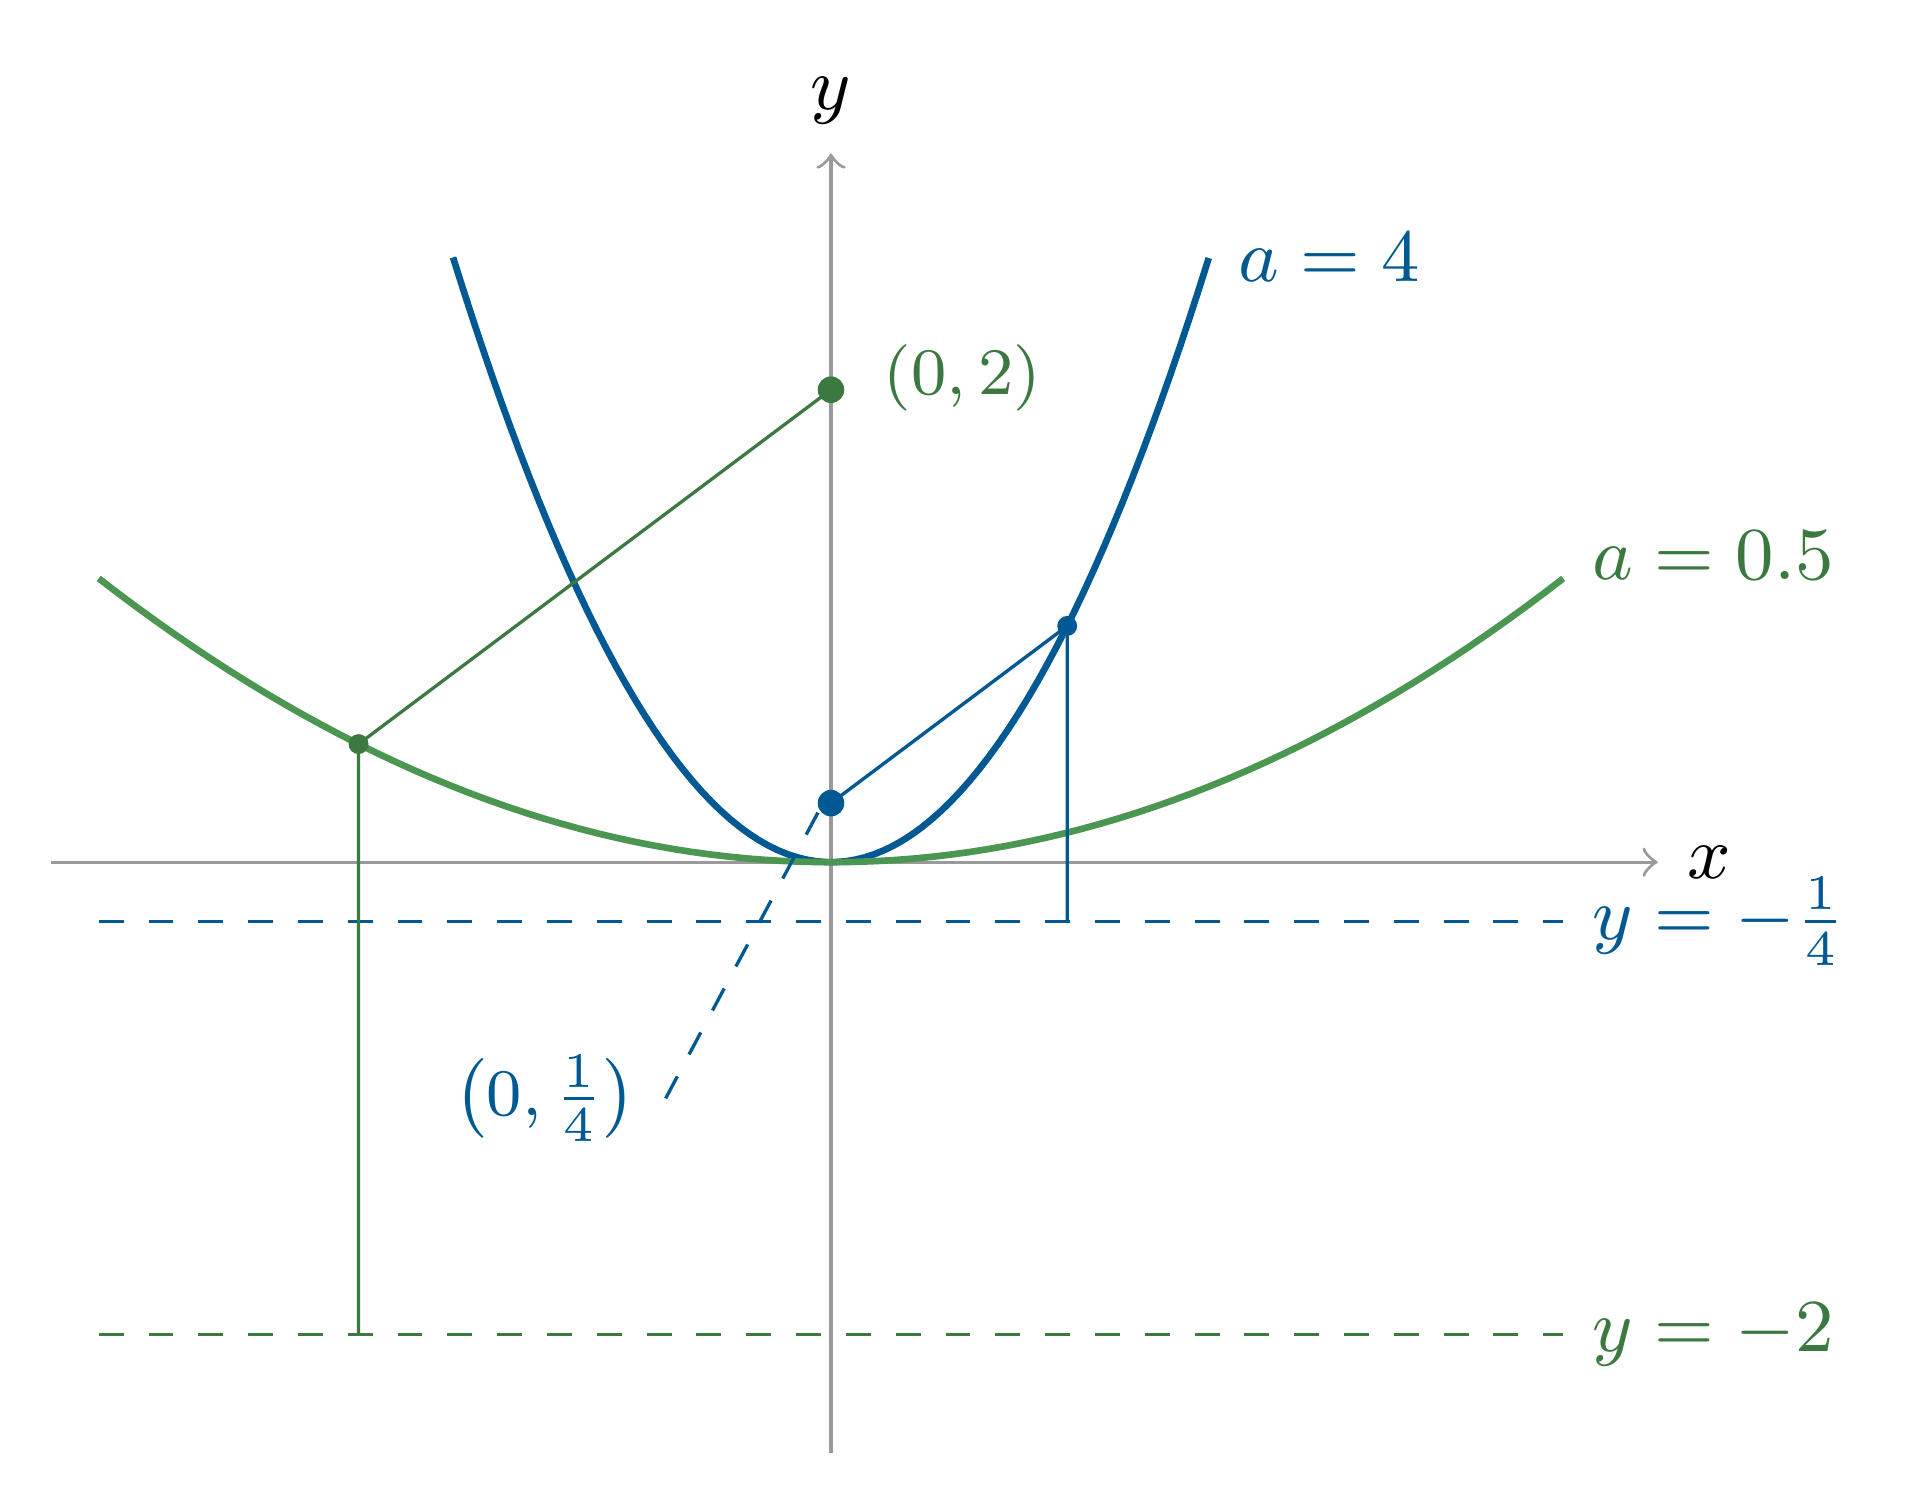
\includegraphics[width=0.49\textwidth]{refl_two_foci.png}
    \caption{Each parabola has its own focus and directrix: $\left(0, \frac{1}{4}\right)$ and $y = -\frac{1}{4}$ for $a = 4$, and $(0, 2)$ and $y = -2$ for $a = 0.5$.}
    \label{fig:refl-two-foci}
\end{figure}

\subsubsection{Reflective Property of a Parabola}

Assume you have a parabola-shaped mirror. A beam of light shot from
the focus will bounce off the mirror in the direction of the axis of
symmetry:
\begin{figure}[H]
    \centering
    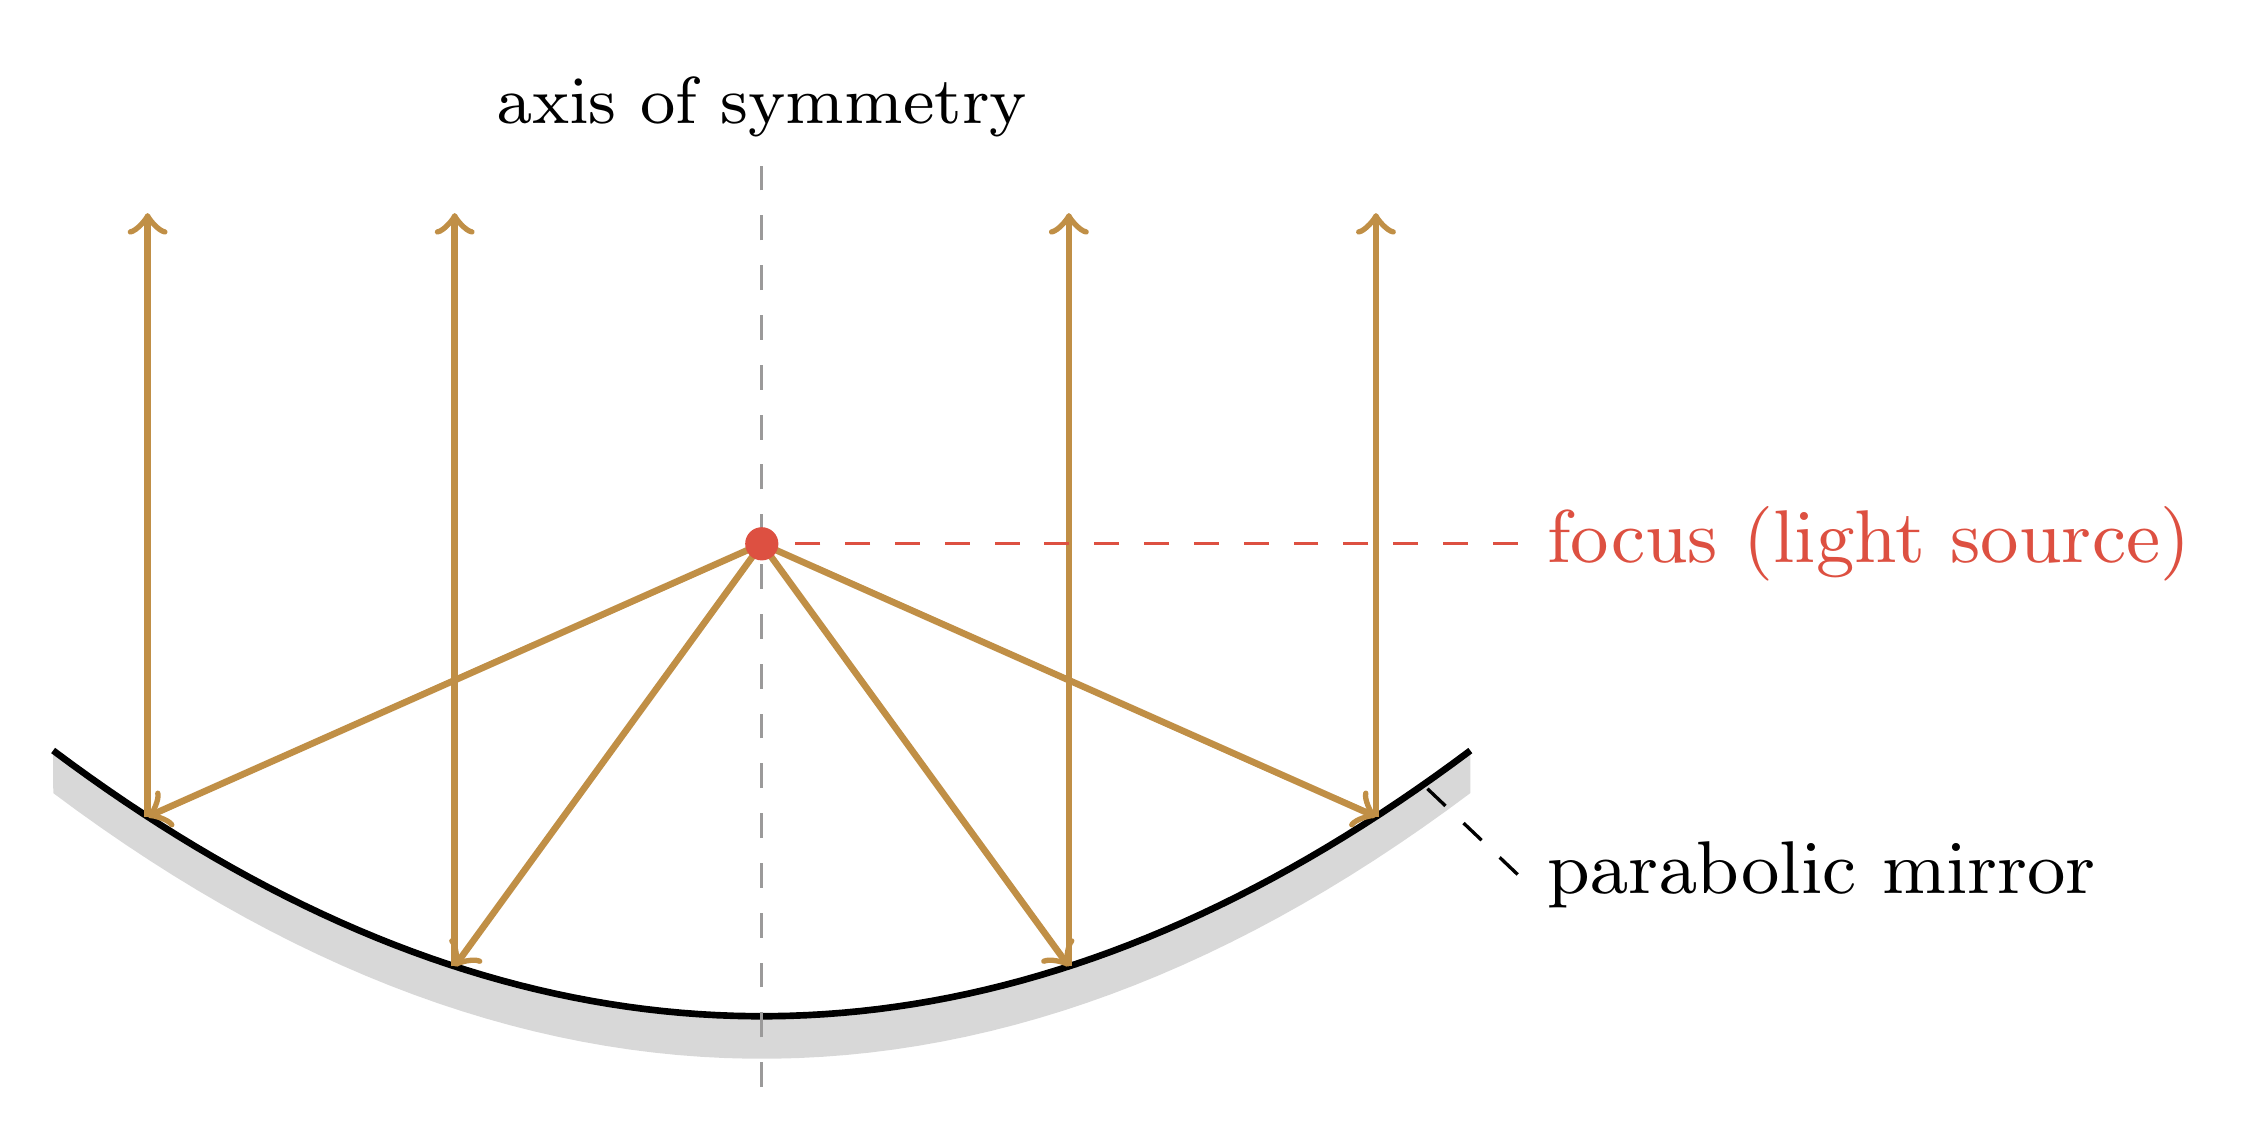
\includegraphics[width=0.58\textwidth]{refl_parabolic_mirror.png}
    \caption{Light leaving the focus of a parabolic mirror reflects parallel to the axis of symmetry.}
    \label{fig:refl-parabolic-mirror}
\end{figure}

This is why your flashlight has a parabolic mirror. The lightbulb is
at the focus, so any photons that hit the mirror are redirected
straight forward.

(Note that in the real world, we use \index{parabolic dish}parabolic dishes: a parabola rotated around its axis of
symmetry.)

The reflection works exactly the same in reverse. There are solar
cookers that are big parabolic mirrors. They let you put a pot on the
focus point. You move the dish until its axis of symmetry is pointed
at the sun.

You will also see a lot of antennas have parabolic dishes. Note that
photons that come in parallel to the axis of symmetry are redirected
to a single point: where the receiver is.
\begin{figure}[H]
  \centering
  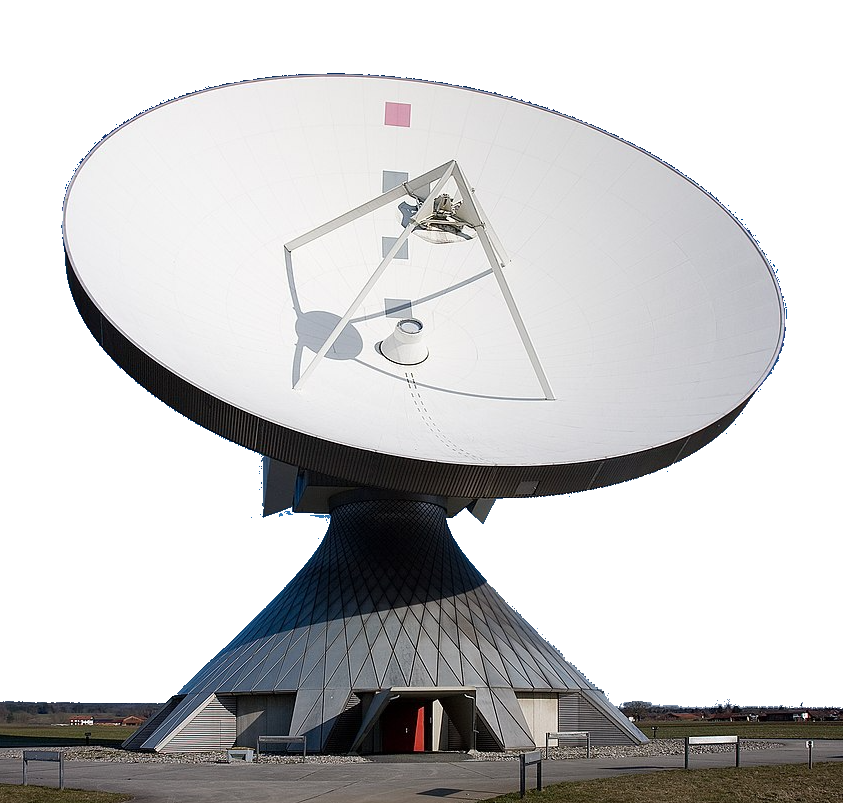
\includegraphics[width=0.7\linewidth]{dish.png}
  \caption{A real life parabolic dish as a satellite.}
  \label{fig:dish}
\end{figure}



Sometimes in a science museum, you will see two parabolic dishes far
apart and pointed at each other. One person speaks with their mouth
at the focus of one. The other person listens with their ear at the
focus of the other. Even though you are very far apart, it sounds like
they are really, really close.
%FIXME figure
\begin{figure}[H]
  \centering
  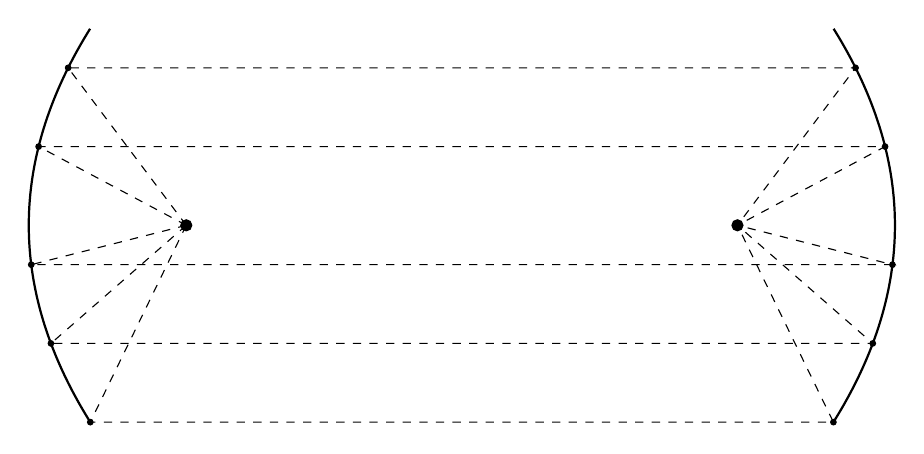
\begin{tikzpicture}
    \coordinate (f1) at (9, 0);
    \coordinate (f2) at (2, 0);
    \coordinate (p1) at (0.125, 1);
    \coordinate (p1d) at (10.875,1);
    \coordinate (p2) at (0.28125,-1.5);
    \coordinate (p2d) at (10.71875, -1.5);
    \coordinate (p3) at (0.5,2);
    \coordinate (p3d) at (10.5, 2);
    \coordinate (p4) at (0.03125, -0.5);
    \coordinate (p4d) at (10.96875, -0.5);
    \coordinate (p5) at (0.78125, -2.5);
    \coordinate (p5d) at (10.21875, -2.5);
    \draw[domain=-2.5:2.5,samples=300,variable=\x, thick]  plot ({0.125*\x*\x},\x);
    \draw[domain=-2.5:2.5,samples=300,variable=\x, thick]  plot ({11 - 0.125*\x*\x},\x);
    \filldraw  (f1) circle (2pt);
    \filldraw  (f2) circle (2pt);
    \filldraw  (p1) circle (1pt);
    \filldraw  (p1d) circle (1pt);
    \draw [thin,dashed] (f2) -- (p1) -- (p1d) -- (f1);
    \filldraw  (p2) circle (1pt);
    \filldraw  (p2d) circle (1pt);
    \draw [thin,dashed] (f2) -- (p2) -- (p2d) -- (f1);
    \filldraw  (p3) circle (1pt);
    \filldraw  (p3d) circle (1pt);
    \draw [thin,dashed] (f2) -- (p3) -- (p3d)--(f1);
    \filldraw  (p4) circle (1pt);
    \filldraw  (p4d) circle (1pt);
    \draw [thin,dashed] (f2) -- (p4) -- (p4d) -- (f1);
    \filldraw  (p5) circle (1pt);
    \filldraw  (p5d) circle (1pt);
    \draw [thin,dashed] (f2) -- (p5) -- (p5d) -- (f1);
  \end{tikzpicture}
  \caption{Two parabolic dishes send waves between each other.}
  \label{fig:parabolicDishes}
\end{figure}

This is because the speaker's parabolic wall focuses the sound energy
in a nice beam the size of the wall pointed straight at the listener's
parabolic wall. The listener's wall focuses the energy of that beam
at the listener's ear.


\section{Refraction}
\subsection{Bending Light at a Boundary}

\index{refraction}The refraction of light is a phenomenon where light changes its direction when it passes from one medium to another. The change in direction is due to a change in the speed of light as it moves from one medium to another. Do not confuse this with rarefaction, which sounds similar and is a similar wave concept for decompression!

\subsection{Snell's Law}
\index{Snell's law}This phenomenon is explained by Snell's law, which states:

\begin{equation}
n_1 \cdot \sin(\theta_1) = n_2 \cdot \sin(\theta_2)
\end{equation}

where:
\begin{itemize}
\item $n_1$ and $n_2$ are the indices of refraction for the first and second media, respectively. The \index{index of refraction}index of refraction is the ratio of, $c$ the speed of light in a vacuum to, $v$ the speed of light in the medium, $n=\frac{c}{v}$. It is a dimensionless quantity. $n \ge 1$ for all materials, such that $n_{\text{vacuum}} = 1$ and $n_{\text{air}} \approx 1$. See a list of all mediums here: \url{https://en.wikipedia.org/wiki/List_of_refractive_indices}
\item $\theta_1$ and $\theta_2$ are the angles of incidence and refraction, respectively. These angles are measured from the normal (perpendicular line) to the surface at the point where light hits the boundary.
\end{itemize}

\begin{figure}[H]
    \centering
    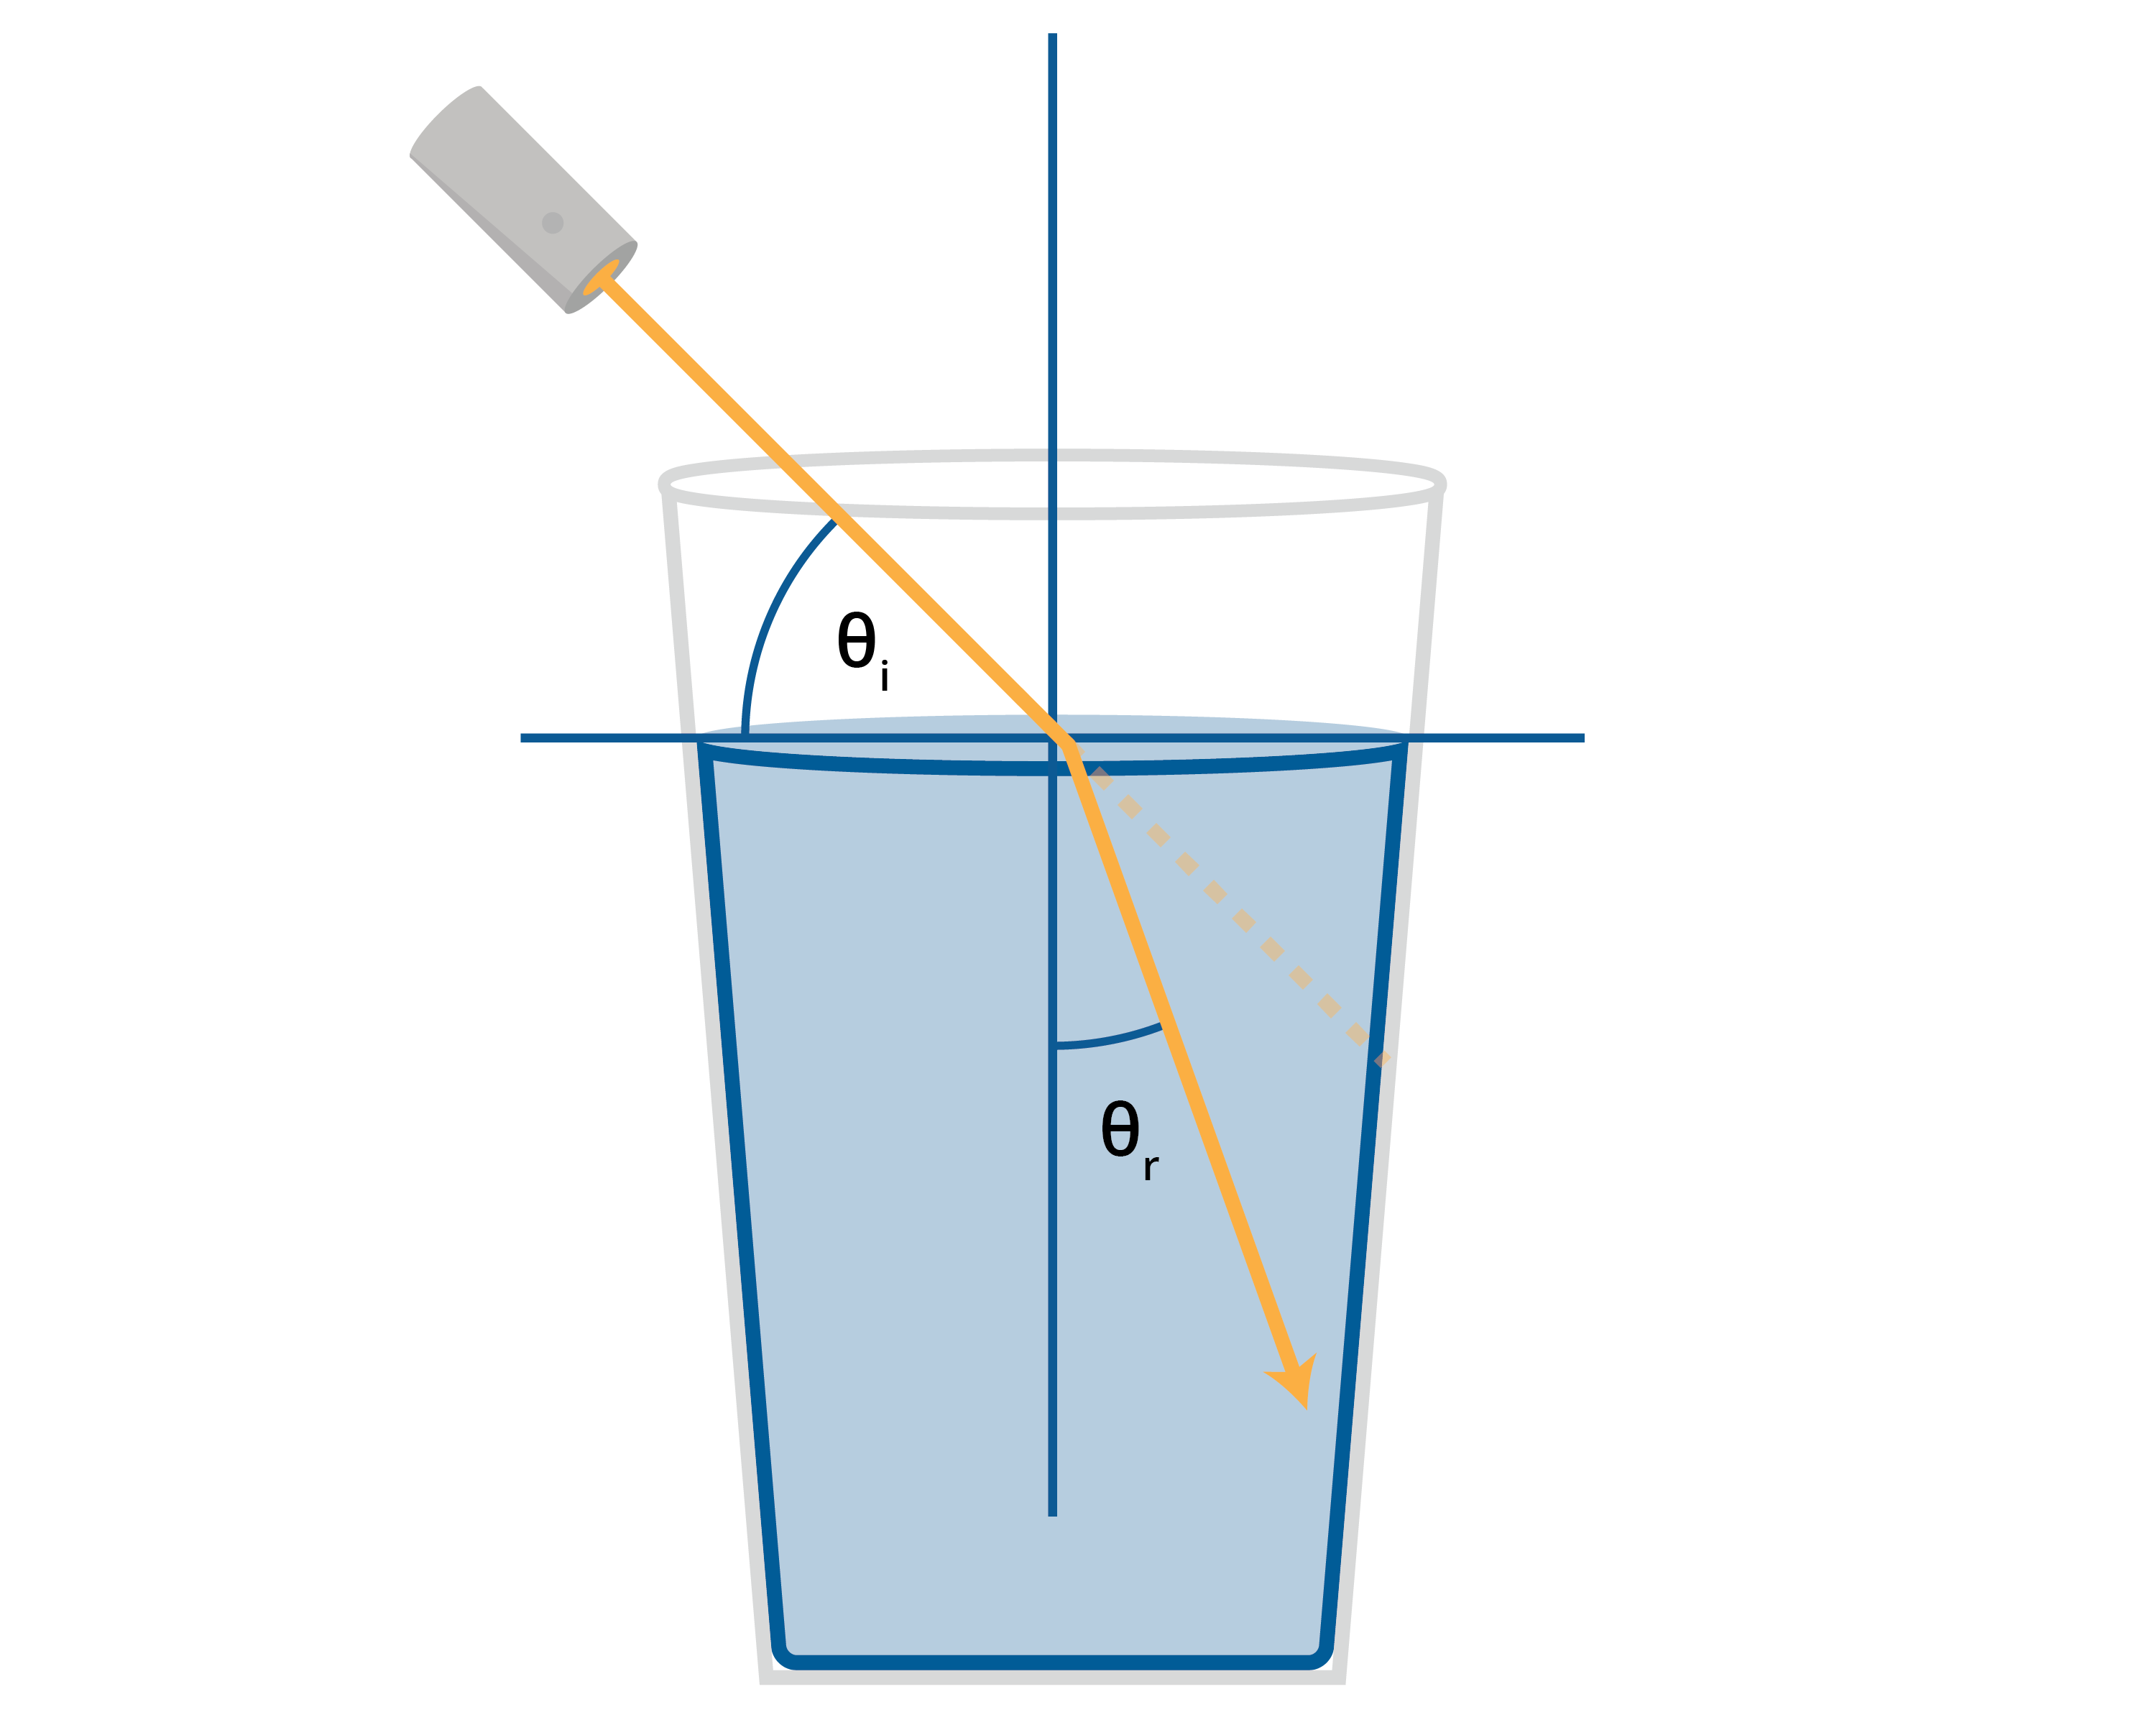
\includegraphics[width=.75\textwidth]{refraction.png}
    \caption{Refraction occurs when light changes the medium it is in.}
    \label{fig:refraction}
\end{figure}

The \index{angle of incidence}angle of incidence ($\theta_1$) is the angle between the incident ray and the normal to the interface at the point of incidence. Similarly, the \index{angle of refraction}angle of refraction ($\theta_2$) is the angle between the refracted ray and the normal.

When light travels from a medium with a lower refractive index to a medium with a higher refractive index, it bends towards the normal. Conversely, when light travels from a medium with a higher refractive index to one with a lower refractive index, it bends away from the normal.

\subsection{Diffraction}


\section{Lenses}
Lenses are optical devices with perfect or approximate axial symmetry
that transmit and refract light, converging or diverging the
beam. There are two main types of lenses, distinguished by their shape
and the way they refract light:\index{lenses}

\begin{itemize}
    \item \textbf{Converging (or Convex) Lenses:}\index{converging lens} These are thicker at
      the center than at the edges. When parallel light rays enter a
      convex lens, they converge to a point called the \index{focal point}focal
      point. Examples of converging lenses include magnifying glasses
      and camera lenses.

      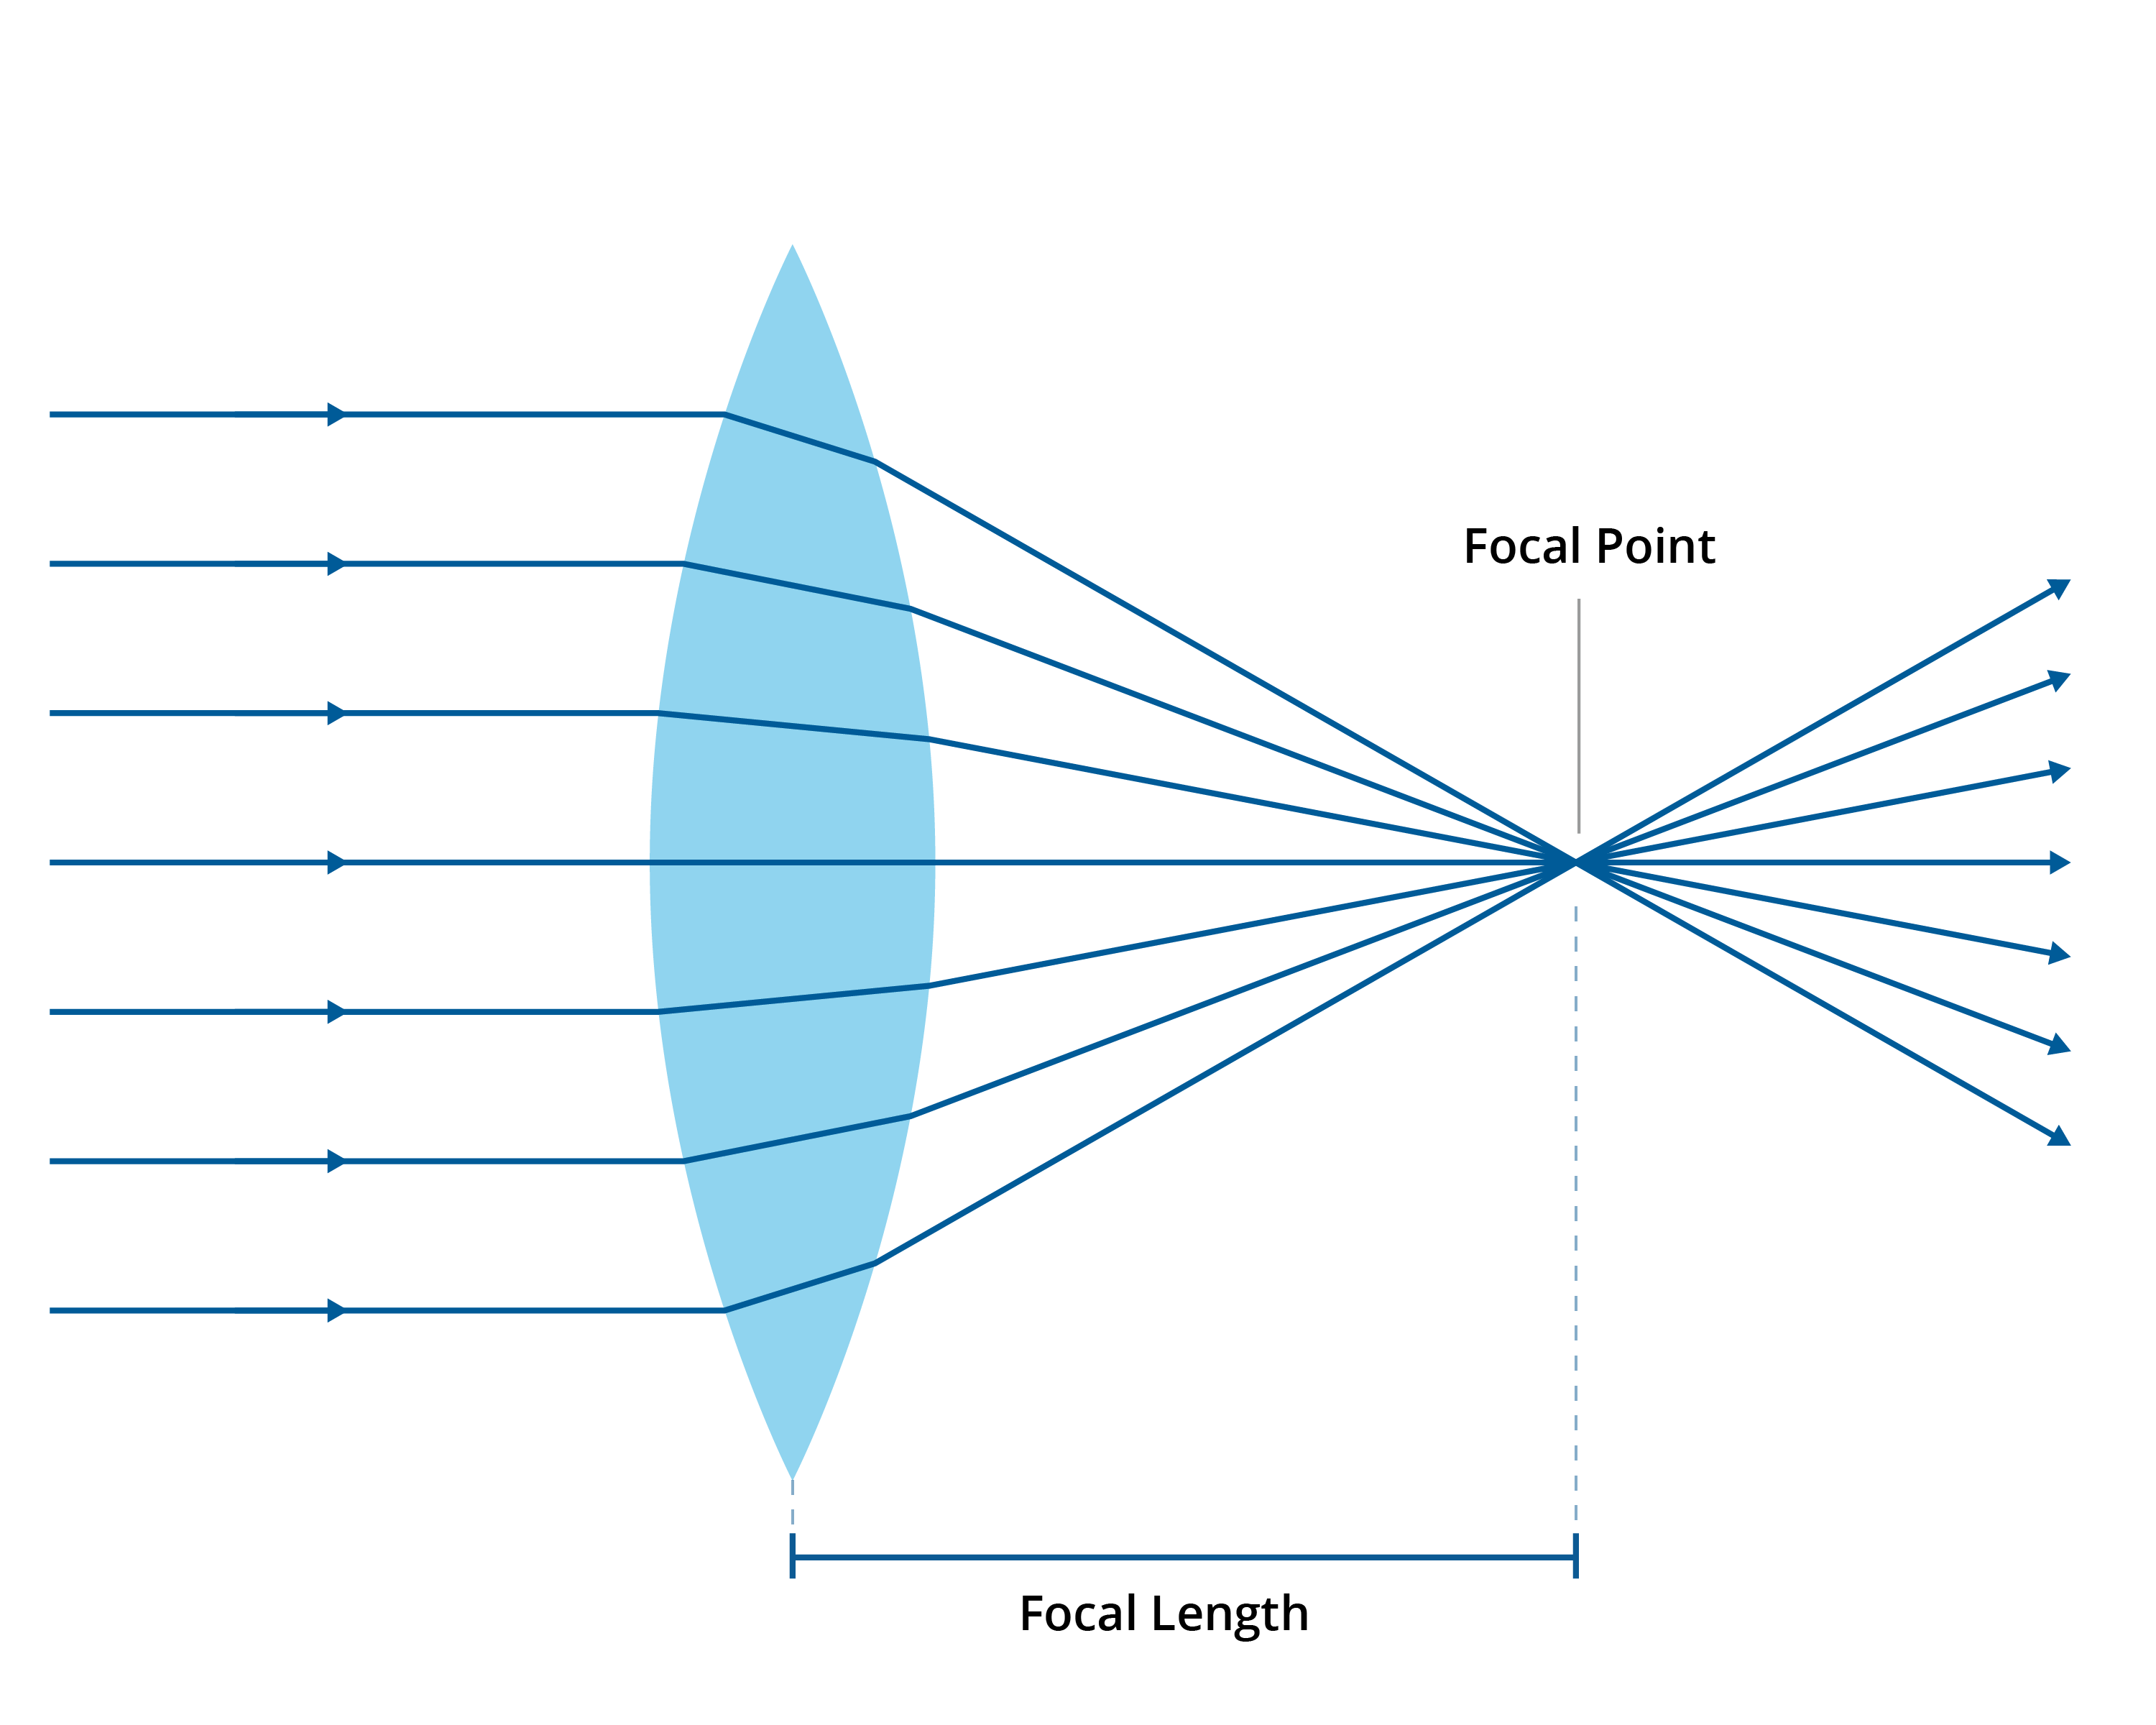
\includegraphics[width=0.5\textwidth]{convex.png}

    \item \textbf{Diverging (or Concave) Lenses:}\index{diverging lens} These are thinner at
      the center than at the edges. When parallel light rays enter a
      concave lens, they diverge or spread out. These lenses are often
      used in glasses to correct nearsightedness.
      
      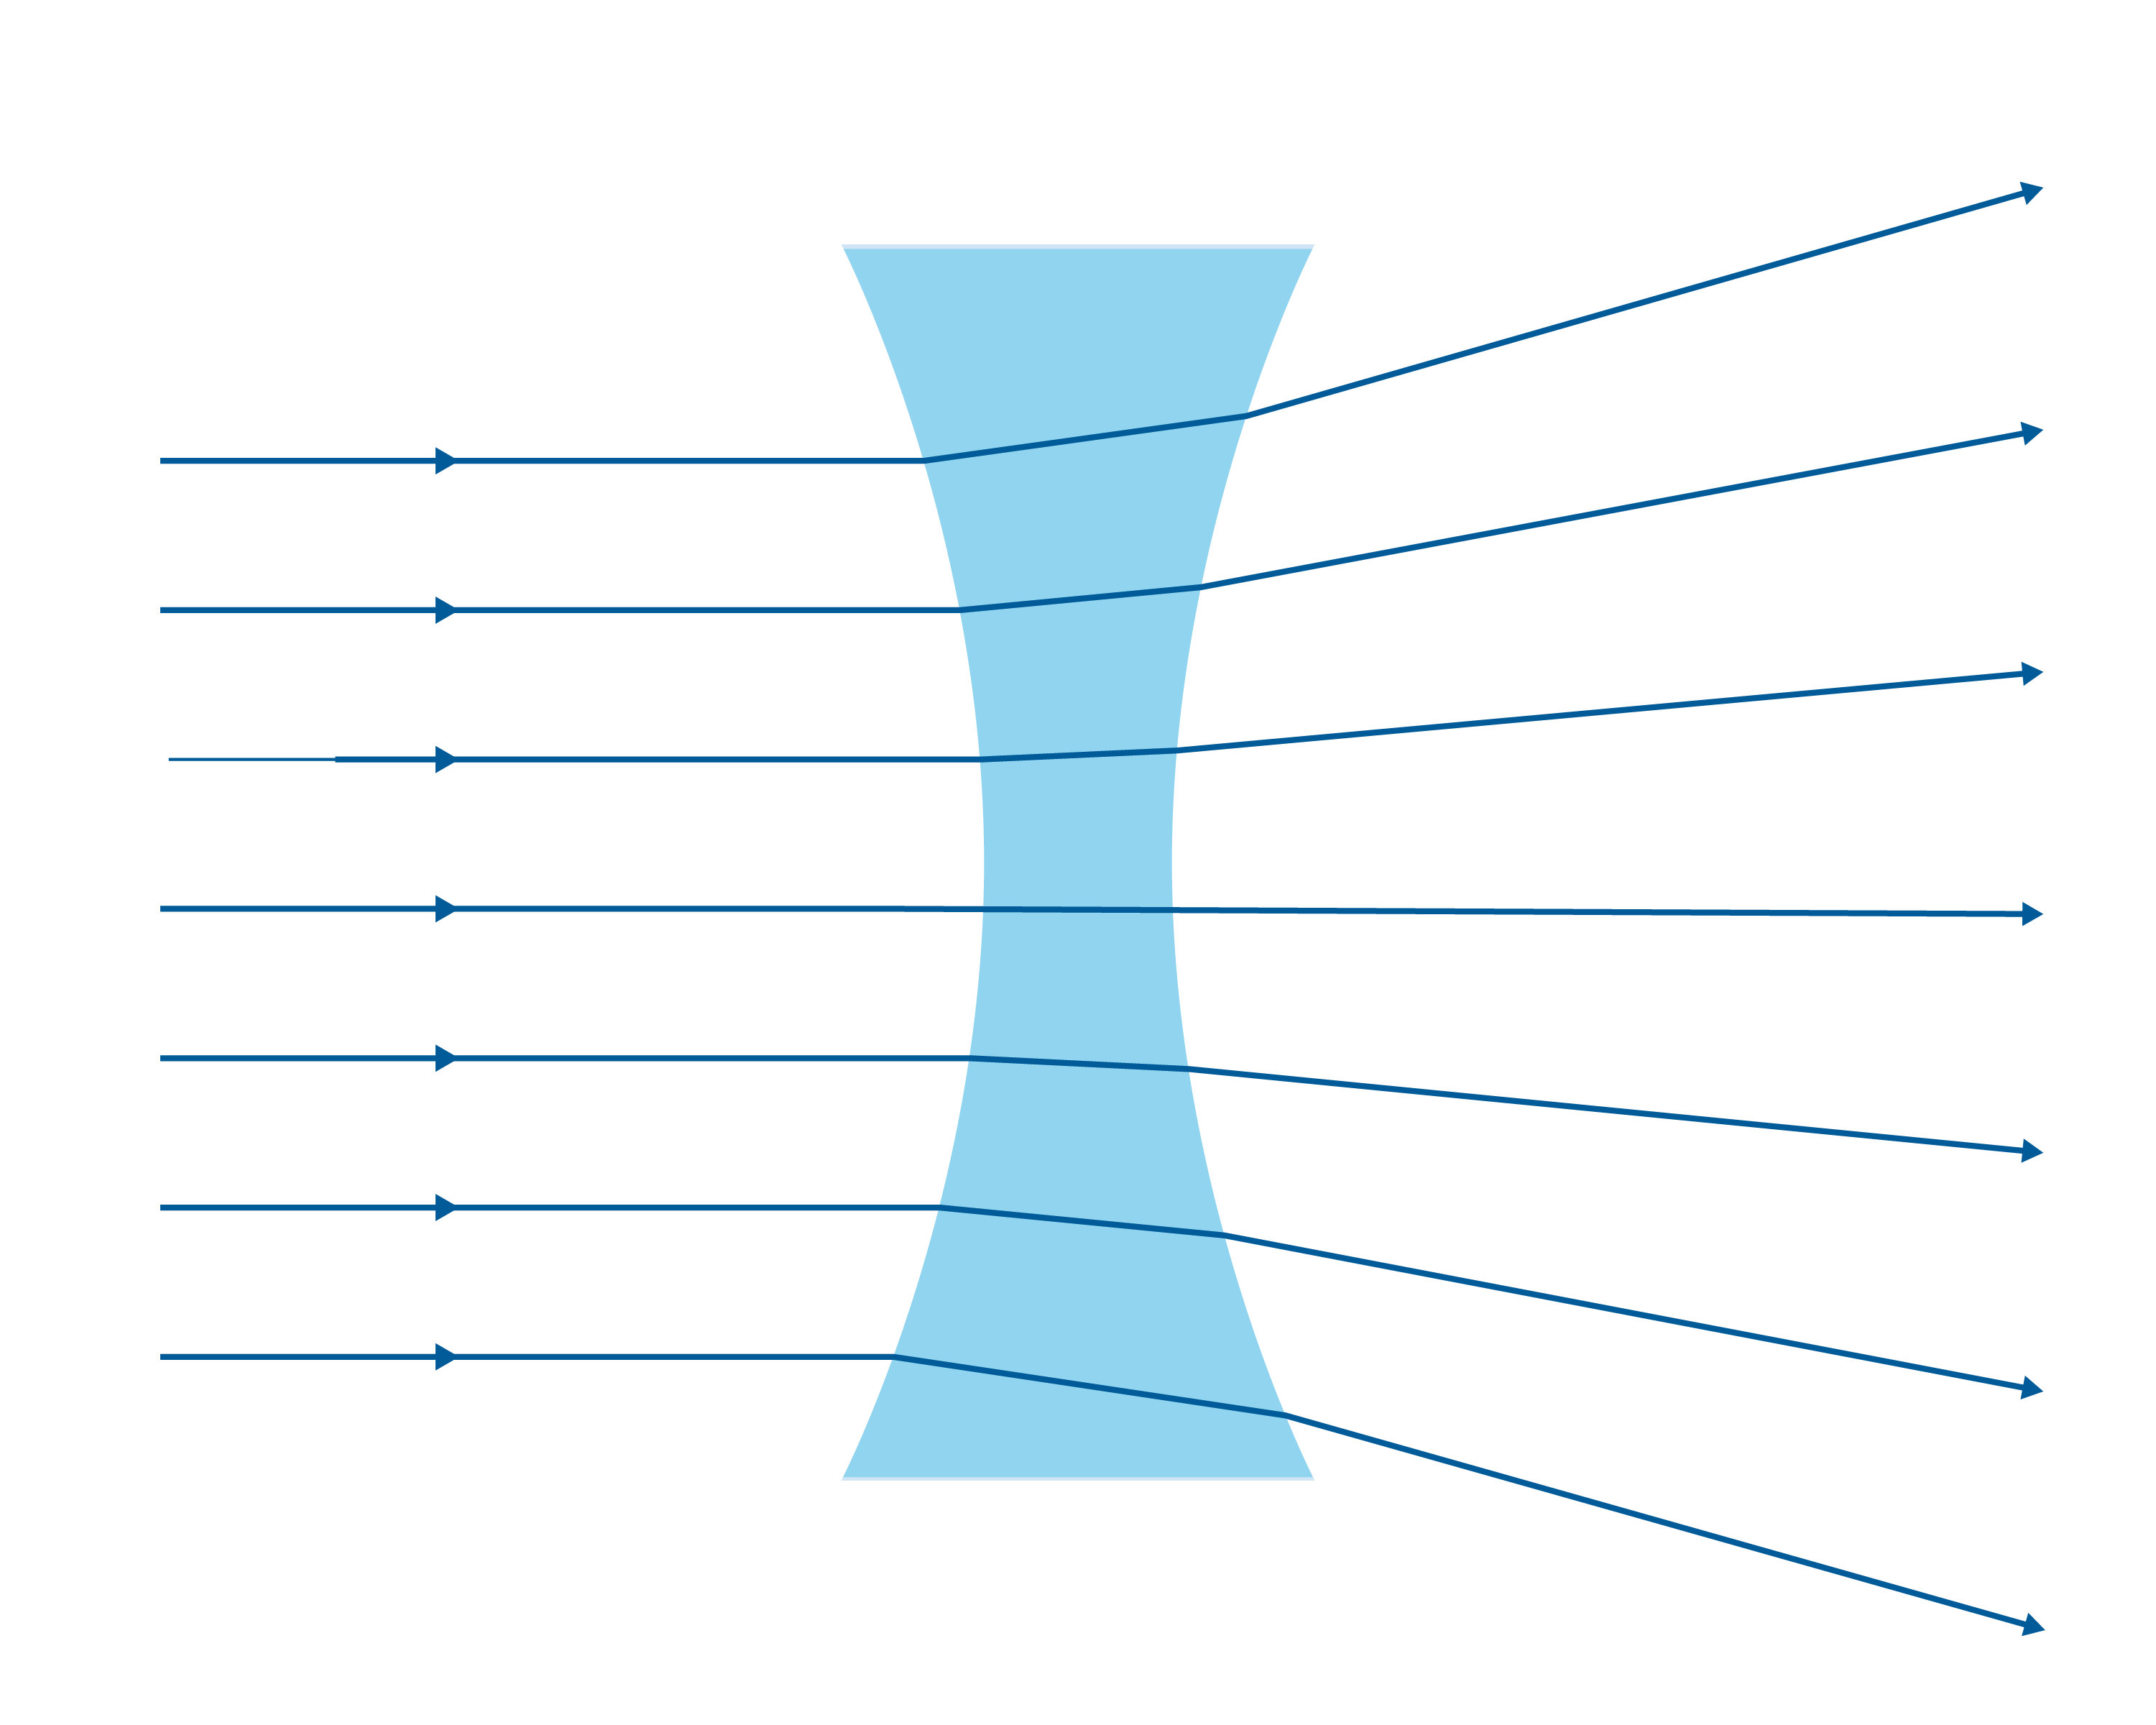
\includegraphics[width=0.5\textwidth]{concave.png}

\end{itemize}

\subsection{Focal Length}

The focal length of a lens is the distance between the center of the
lens and the focal point. It is determined by the lens shape and the
refractive index of the lens material. For a converging lens, the
focal length is positive; for a diverging lens, the focal length
is negative.\index{focal length}

\subsection{The Lens Equation}

Thin lenses follow the same relation as mirrors:
$$\frac{1}{f} = \frac{1}{d_o} + \frac{1}{d_i}$$
where $d_o$ is the distance from the object to the lens and $d_i$ is the distance from the lens to the image. A converging lens has $f > 0$, and a diverging lens has $f < 0$.

\textbf{Worked example: a converging lens.} A converging lens has $f = 10$ cm. An object is $30$ cm from the lens. Then $$\frac{1}{d_i} = \frac{1}{10} - \frac{1}{30} = \frac{2}{30}, \qquad d_i = 15 \text{ cm}$$ The image is real, on the other side of the lens, and it is smaller than the object.

\subsection{Refractive Index}

The refractive index of a material is a measure of how much the speed
of light is reduced inside the material. The refractive index $n$ of a
material is given by the ratio of the speed of light in a vacuum $c$
to the speed of light $v$ in the material:\index{refractive index}

\[
n = \frac{c}{v}
\]

The refractive index affects how much a light ray changes direction,
or refracts, when entering the material at an angle. A higher
refractive index indicates that light travels slower in that medium,
and the light ray will bend more towards the normal.

Lenses work by refracting light at their two surfaces. By choosing the
right lens shape and material, lenses can be designed to bring light
to a focus, spread it out, or perform more complex transformations.

\begin{Exercise}[title={Object Moved Closer}, label=opt4]
A concave mirror has focal length $f = 10$ cm. An object is placed $20$ cm in front of the mirror. Where is its image?
\end{Exercise}
\begin{Answer}[ref=opt4]
$\frac{1}{d_i} = \frac{1}{10} - \frac{1}{20} = \frac{1}{20}$, so $d_i = 20$ cm.
\end{Answer}
